\providecommand{\econtexRoot}{}
\renewcommand{\econtexRoot}{.}
\providecommand{\econtex}{\econtexRoot/texmf-local/tex/latex/econtex}
\providecommand{\econtexSetup}{\econtexRoot/texmf-local/tex/latex/econtexSetup}
\providecommand{\econtexShortcuts}{\econtexRoot/texmf-local/tex/latex/econtexShortcuts}
\providecommand{\econtexBibMake}{\econtexRoot/texmf-local/tex/latex/econtexBibMake}
\providecommand{\econtexBibStyle}{\econtexRoot/texmf-local/bibtex/bst/econtex}
\providecommand{\notes}{\econtexRoot/texmf-local/tex/latex/handout}
\providecommand{\handoutSetup}{\econtexRoot/texmf-local/tex/latex/handoutSetup}
\providecommand{\handoutShortcuts}{\econtexRoot/texmf-local/tex/latex/handoutShortcuts}
\providecommand{\handoutBibMake}{\econtexRoot/texmf-local/tex/latex/handoutBibMake}
\providecommand{\handoutBibStyle}{\econtexRoot/texmf-local/bibtex/bst/handout}

  
\documentclass[titlepage]{\econtex}\providecommand{\texname}{Dissertation-Proposal}


\providecommand{\EqDir}{Equations}
\providecommand{\FigDir}{Figures}
\providecommand{\CodeDir}{Code}
\providecommand{\CalibrationDir}{Calibration}
\providecommand{\TableDir}{Tables}
\providecommand{\ApndxDir}{Appendices}

\usepackage{subfiles}

\providecommand{\onlyinsubfile}{}
\providecommand{\notinsubfile}{}
\renewcommand{\onlyinsubfile}[1]{}
\renewcommand{\notinsubfile}[1]{#1} 


\usepackage{\econtexSetup}\usepackage{\econtexShortcuts}\usepackage{makecell} 
\renewcommand{\util}{\mathrm{u}}
% replace PF-FHWC with just FHWC
\renewcommand{\InvEpShkInv}{\hat{\pShk}}
%\renewcommand{\InvEpShkInv}{\check{\pShk}}
\renewcommand{\PGroAdj}{\hat{\PGro}}
\renewcommand{\PatPGroAdj}{\text{\pmb{\Thorn}}_{\PGroAdj}}
% get rid of \DiscAlt
\renewcommand{\PGrouAdj}{\ensuremath{\hat{\hat{\PGro}}}}
\renewcommand{\pGrouAdj}{\ensuremath{\hat{\hat{{\pGro}}}}}
\renewcommand{\DiscAltuAdj}{\ensuremath{\hat{\hat{\beth}}}}
\renewcommand{\uInvEpShkuInv}{\hat{\hat{\psi}}}
\renewcommand{\pNotZero}{(1-\pZero)}
\providecommand{\YLevBF}{\ensuremath{\mathbf{Y}}}


\provideboolean{Shorter}
\setboolean{Shorter}{true}
\setboolean{Shorter}{false}
\providecommand{\ShorterYN}{\ifthenelse{\boolean{Shorter}}}
\usepackage{rotating}\usepackage{subfigure}

%%%%%%%%%%%%%%%%%%%%%%%%%%%%%%%
%PACKAGES I ADDED MYSELF
\usepackage[capposition=top]{floatrow}
\usepackage{float}
\newcommand{\plotheight}{0.27}
\newcommand{\plotwidth}{1.0}


%%%%%%%%%%%%%%%%%%%%%%%%%%%%%%%
\hypersetup{pdfauthor={William Du <wdu9@jhu.edu>},
            pdftitle={Dissertation Proposal},
            pdfkeywords={Heterogenous Agents, marginal propensity to consume, Nominal Rigidities, buffer-stock saving, permanent income hypothesis},
            pdfcreator = {wdu9@jhu.edu}
}

\begin{document}\bibliographystyle{\econtexBibStyle}
\renewcommand{\onlyinsubfile}[1]{}\renewcommand{\notinsubfile}[1]{#1} 

\hfill{\tiny \texname.tex, \today}

\begin{verbatimwrite}{\texname.title}
Theoretical Foundations of Buffer Stock Saving
\end{verbatimwrite}


\title{ The Distribution of Wealth, Precautionary Saving, and the Business Cycle}

\author{William Du\authNum}



\keywords{Precautionary Saving, Heterogeneous Agents, Incomplete Markets, Beliefs, Search and Matching}




\maketitle 


\hypertarget{abstract}{}
\begin{abstract}
In a heterogenous agents New Keynesian model with search and matching frictions and beliefs on job finding, I quantify the role of precautionary saving over the business cycle.
%This dissertation proposes studying the implications of expectations data on job transition probabilities on the role of precautionary saving over the business cycle. 

\end{abstract}


\begin{authorsinfo}
\name{Contact: \href{mailto:wdu9@jhu.edu}{\texttt{wdu9@jhu.edu}}}
\end{authorsinfo}

\thanks{ }

\titlepagefinish


\newtheorem{defn}{Definition}
\newtheorem{theorem}{Theorem}

\hypertarget{Introduction}{}
\section{Introduction}

\label{sec:intro}

%  - Unemployment risk channel important for business fluctuations and UI

%  - This channel works through precautionary saving. Precautionary saving is dictated by household expectations.

%  -  Let us quantify the role of unemployment risk channel with expectations data

%  - What are the determinants of the magnitude of the precautionary channel and what causes it to amplify

% When is the precautionary motive strong? If there is a rise in uncertainty, when will the effects be large and when will it be weak?


%Under what economic conditions are business cycle fluctuations sensitive to elevated unemployment risk? 


% - First paragraph , understanding the precautionary channel is important because it is a key mechanism through which unemployment insurance works through

%study the sensitivity of precautionary saving to heightened uncertainty
% In what circumstances is the precautionary channel la? 

The past decade has seen an eruption of research on the importance of household uncertainty over the business cycle. Increases in household uncertainty, in the form of heightened income or unemployment risk, have shown to generate sizable business cycle fluctuations. Although the effects of uncertainty are transmitted through the precautionary channel\footnote{The channel through which business cycle fluctutations are amplified from increases in precautionary saving.}, few papers study the sensitivity of the precautionary channel to economic conditions. Given precautionary saving is a central mechanism to the effectiveness of unemployment benefits (\cite{Kekre2021}), it is critical to understand the determinants of the magnitude of the precautionary channel in the design of unemployment insurance policy.\\

In this paper, I quantify the precautionary channel and study its sensitivity to the distribution of liquid wealth in a Heterogeneous Agent New Keynesian(HANK) model with Search and Matching (SAM) frictions and beliefs on job finding probabilities. In particular, I study the determinants of the magnitude of the precautionary channel over the business cycle with a focus on the distribution of liquid wealth. Since precautionary saving is dictated by household expectations, I allow households to form beliefs on job finding expectations to capture the underreaction in job finding expectations found in recent work by \cite{mueller2021job} and Du, Qiu, and Wang (2022). The model features idiosyncratic income shocks to generate a realistic distribution of wealth in order to both study the relationship between precautionary saving over the cross section of wealth and to match the empirical dynamic consumption response out of unanticipated income shocks documented in \cite{Fagereng2021}. A distribution of liquid wealth that contains a significant share of households who hold little liquidity (but are not  constrained) is necessary to generate an empirically consistent dynamic consumption response and, as a consequence, vital to the general equilibrium transmission of shocks with nominal rigidities (\cite{auclert2018intertemporal}). \\

 
In my main result so far, I find the magnitude of the precautionary channel following a monetary policy contraction to rise exponentially with the persistence of the policy shock. This is because the precautionary channel depends on both the persistence of heightened unemployment risk and the interaction of this persistence with the empirically consistent dynamic consumption response of households. When households perceive unemployment risk to rise for a longer duration, they accumulate larger precautionary savings leading to a dramatic decline in aggregate consumption and, as a consequence, a severe rise in the unemployment rate. These fluctuations are amplified as the consumption response of newly unemployed households persist beyond the initial impact of the unemployment spell due to the persistence in the empirical dynamic consumption response. Overall, this result emphasizes the importance of the duration of heightened unemployment risk in the magnitude of the precautionary channel. With regards to unemployment insurance policy, this result motivates the duration of unemployment benefit extension as opposed to the magnitude of benefits in the efficient stablization of macroeconomic aggregates. \\

%The strength of a macroeconomic stabilization policy that work through household's expectations of unemployment risk should have persistence in mind.

%The effectiveness of unemployment insurance policy in stabilizing aggregate demand is strongly dependent on the persistence of the insurance offered





%Although precautionary saving operates through households expectations of their future income, no work has used expectations data to quantify the role of precautionary saving. Considering the expansive literature on the surrounding biases in the formation of expectations, the quantitative implications of the precautionary saving channel may differ substantially when household beliefs are disciplined by expectations data.  In this paper, I use expectations data on job finding probabilities to quantify the role of precautionary saving over the business cycle and study its determinants. 



%Establish size of precautionary channel, 
 
% Channel is strongly dependent on the peristence of the shock
 
% The reason being is that precaution is sensitiive to the duration of heightened unemployment risk and interaction of this sensitivity with persistent IMPCs

%Thus, in my job market paper, I aim to use expectations data on job transition probabilities to quantify the role of precautionary saving over the business cycle. Furthermore, I look to understand how the quantitative consequences of precautionary saving differ when households expectations are disciplined by expectations data on job transition probabilities as opposed to data on the actual job transition probabilities. For the moment, the goal is to capture the quantitative implications of biases inherent in the expectations data and how they influence precautionary savings to induce business cycle fluctuations instead of taking a theoretical stance on how or why these biases are formed. \\

%\subsection{Framework To Solve Problem}
%\label{subsec:Framework To Solve Problem}


%I solve a Heterogeneous Agent New Keynesian(HANK) model with Search and Matching (SAM) frictions, and beliefs on job transition probabilities. In the model, households face uninsurable stochastic unemployment risk dictated by job finding and job separating probabilities.The true job transition probabilities are unobserved by households and instead households form beliefs on these probabilities.  Since precautionary saving is dictated by households expectations, it is important to capture how expectations on job transition probabilities evolve over the business cycle. Recent work has demonstrated that household job finding expectations underreact in comparison to the true job finding probability (\cite{mueller2021job}, Du, Qiu, and Wang 2022).  I therefore add beliefs on job finding probabilities to capture the underreactive bias present in the data. I do not not take a stance on how beliefs are formed theoretically. Beliefs will be updated according to an empirical relationship between the expectations data on job transition probabilities and the actual job transition probabilities. The aim is to capture what the expectations data implies as opposed to how households form expectations on job transition probabilities. 

%To quantify the role precautionary saving with expectations data,  I solve a Heterogeneous Agent New Keynesian(HANK) model with Search and Matching (SAM) frictions, and beliefs on job transition probabilities. In the model, households face uninsurable stochastic unemployment risk dictated by job finding and job separating probabilities.The true job transition probabilities are unobserved by households and instead households form beliefs on these probabilities. I do not not take a stance on how beliefs are formed theoretically. Beliefs will be updated according to an empirical relationship between the expectations data on job transition probabilities and the actual job transition probabilities. The aim is to capture what the expectations data implies as opposed to how households form expectations on job transition probabilities. \\

%%The addition of search and matching frictions not only provide a foundation to accommodate expectations data on job transition probabilities but also allow for a micro-founded model of counter-cyclical unemployment risk. The HANK and SAM literature has documented that the interaction between risk aversion, nominal rigidities, and search frictions produces counter cyclical unemployment risk that amplifies fluctuations in aggregate demand. Intuitively, a fall in output reduces labor demand which in turn reduces the number of vacancies leading job finding probabilities to fall and job separating probabilities to rise inducing a precautionary savings motive that causes a further decline in consumption and, equivalently, output. This theory is consistent with the work of \cite{leduc2016uncertainty}, who find that the effects of macroeconomic uncertainty operate partly through an aggregate demand channel and the findings of \cite{guvenen2014nature}, who document that earnings growth exhibits pro-cyclical skewness implying severe negative events are more likely during recessions. \\

%%In addition, households face permanent and transitory income shocks to produce a realistic model of households that can match the empirical distribution of wealth and generate realistic fluctuations in aggregate consumption. Given the importance of aggregate demand in the transmission of the precautionary channel, it is vital to have a realistic model of household behavior.  Recent research in the HANK literature has emphasized the importance of the distribution of wealth in producing realistic fluctuations in aggregate consumption\footnote{\cite{auclert2018intertemporal}, \cite{patterson2019matching} , \cite{kaplan2018monetary}}. For instance, \cite{auclert2018intertemporal}  emphasize the role of the intermediately constrained households (households that are nearly hand to mouth) in generating persistence in the dynamics of aggregate consumption that cannot be replicated by a TANK model. Further, \cite{auclert2019monetary} establishes the existence of redistribution channels in the transmission of monetary policy exclusive to HANK models. Confirming the empirical significance of this channel by using administrative data from Denmark, \cite{crawley2020consumption} demonstrate some of these redistributive channels to be substantially more important in explaining consumption growth than the intertemporal substitution channel. In a structural model, the strength of these redistributive channels are functions of the cross sectional distribution of MPCs and therefore the cross sectional distribution of wealth. Moreover, \cite{heathcote2018wealth} show that households with lower liquid wealth exhibit increased sensitivity in their precautionary motive when faced with heightened unemployment risk. In summary, the distribution of wealth plays an essential role in shaping the response of aggregate consumption and the share of the precautionary motive therefore permanent and transitory income shocks are included. \\



%Two points for what you can do to relate this to data:
%- (DO experiments in past comparing times in history where there was a persistent shock vs a non persistent shock, some time in past might have had large shock, may explain amplification during that time, or why saving rate was so large)
%- How can this persistence, this result guide the design of policy.
%- how does announcement window of UI affect macroaggregates, so on long annoucnement saying we will extend benefits for 18 months, as opposed to say , we will extend benefits for the first 9 months, then after 9 months say the same thing, the effect will be different.


%The core contribution of this project is the use of expectations data to quantify the role of unemployment risk and precautionary saving over the business cycle. More broadly, this paper is the first to discipline household expectations with expectations data in the study of the effects of uncertainty over the business cycle. The results of this project may motivate the management of unemployment expectations in the design of stabilization policy, especially if these expectations are subject to pervasive biases that amplify business cycle fluctuations. \footnote{Indeed, unemployment expectations have been shown to be robustly correlated with spending (\cite{carroll1997unemployment}). Further, \cite{pedemonte2020fireside} demonstrates that during the Great Depression regions of America with increased exposure to President Roosevelt's fireside chats saw significant increases in spending on durable goods. This is notable as Roosevelt's fireside chats highlighted the introduction of unemployment benefits and other New Deal Legislation suggesting the importance of managing unemployment expectations on stimulating consumer behavior.}\\


The rest of the paper is as follows. Section 2 details a literature review. Section 3 describes the data. Section 4 presents a preliminary model to be disciplined by expectations data. Section 5 details my next steps in the research process and finally section 6 details possible interesting extensions. 

\hypertarget{Literature Review}{}
\section{Literature Review}

The core contribution of this paper is both the inclusion of a realistic distribution of wealth to study the sensitivity of precautionary saving and the evaluation of this sensitivity over the cross section of liquid wealth. \\

This paper contributes to the literature on the role of unemployment risk over the business cycle.  This literature emphasizes the interaction between nominal rigidities, search frictions, and incomplete markets to generate counter-cyclical unemployment risk, and thus countercyclical precautionary savings, that amplify changes in aggregate demand  (\cite{den2018unemployment}, \cite{leduc2016uncertainty}, and \cite{ravn2017job}). Within this literature, work by \cite{challe2017precautionary} do quantify the precautionary channel but do not feature a thorough distribution of wealth to match the dynamic consumption response nor study the sensitivity of precautionary savings. In comparison to these papers, I emphasize the sensitivity of the precautionary mechanism at the center of these papers. Works by \cite{Graves2022} and \cite{broer2021unemployment} do emphasize the factors that amplify the precautionary channel however both works do not focus on the sensitivity of precautionary saving across the distribution in liquid wealth. In particular, \cite{broer2021unemployment} quantify the precautionary channel in a tractable HANK and SAM model that assumes a degenerate distribution of wealth and focus on the role job separations and the supply side implications of sluggish vacancies on the strength of the precautionary channel. \cite{Graves2022} constructs a carefully calibrated HANK and SAM model that features realistic a distribution of wealth and finds the flight to liquidity mechanism induced by heightened unemployment risk to amplify the precautionary channel. His analysis captures the indirect importance of the distribution of liquidity on the amplification of the precautionary channel. I instead look to study how households build precautionary savings in direct response to heightened uncertainty across the distribution of liquidity.  \cite{heathcote2018wealth} emphasize the relationship between liquid wealth and the sensitivity of precautionary saving to heightened uncertainty. Their analysis, however, concerns the overall level of liquid wealth in the economy and studies a highly stylized model of precautionary saving in steady states.\\

This paper also contributes to the HANK literature that emphasize the distribution of wealth in producing realistic dynamic MPCs \cite{auclert2018intertemporal} and realistic transmission mechanisms to monetary policy \cite{kaplan2018monetary, auclert2019monetary}. Instead of studying the consumption responses across the distribution of wealth, I contribute to this literature by studying the precautionary responses to heightened uncertainty across the distribution of wealth.\\


%%For instance, using an estimated quantitative HANK and SAM model, \cite{challe2017precautionary} demonstrate the significance of this precautionary channel by illustrating that the fall in aggregate consumption during the Great Recession would have been 1.75 times smaller without the effects of precautionary savings (-3.5 percent drop in consumption in the data, and they find a -2 percent drop in their counterfactual experiment without precautionary savings). With respect to how HANK and SAM models influence monetary policy, \cite{challe2020uninsured} finds that negative supply shocks call for interest rate cuts due to the amplifying effect of precautionary savings on aggregate demand.  Moreover, \cite{gornemann2016doves} find that households prefer policy focused on unemployment stabilization even if it incurs deviations from price stability due to the amplifying effects of precautionary savings. In regards to quantifying unemployment risk, \cite{broer2021unemployment} add endogenous job separations (typically assumed exogenous in this literature) and sluggish vacancy creation to a HANK and SAM model to produce empirically consistent co-movements between job transition probabilities and to quantify the unemployment risk channel: the difference in the response of unemployment between a model with incomplete markets and and a model with complete markets. They find the unemployment risk channel to account for 35 percent of the variance in unemployment after a TFP shock. Effectively, the unemployment risk channel, as they define it, is the consequence of precautionary savings and therefore their paper is closest to this project. In contrast to \cite{broer2021unemployment}, I look to quantify how the consequences of precautionary savings differ when using expectations data. In addition, since countercyclical income risk operates through aggregate demand to amplify unemployment risk, the response of aggregate consumption is crucial in quantifying this channel. Therefore this project necessitates a model of realistic household behavior with thorough heterogeneity as the HANK literature has shown the importance of the distribution of wealth in explaining fluctuations in aggregate consumption. Few HANK and SAM models generate meaningful heterogeneity across the distribution of wealth. Instead, the literature on countercyclical income risk makes strong assumptions to allow for a degenerate distribution of wealth for tractability and transparency in the mechanisms within the model. Overall, I contribute to the HANK and SAM literature by introducing expectations data on job transition probabilities to quantify the underlying precautionary savings channel/unemployment risk channel that dictates all its results and by being the second paper (first paper to do so is \cite{gornemann2016doves}) to introduce a realistic model of household behavior to the HANK and SAM framework.


\hypertarget{Empirical Evidence of Underreactive Job Finding Expectations}{}
\section{Empirical Evidence of Underreactive Job Finding Expectations}

This section summarizes the findings of Du, Qiu, and Wang (2022) that discipline the job finding expectations of households in the model. In our work, we impute expectations on job finding probabilities from the Survey of Consumer Expectations beginning in 1978 using expectations data from Michigan Survey of Consumer Expectations(MSE) and other real time macroeconomic variables. We find our imputed job finding series is strongly correlated with the realized job finding probability yet is less volatile. Our results suggests households underreact in their job finding expectations to changes in macroeconomic condition in comparison to the realized job finding probability.


\subsection{Data}
\label{subsec:Data}

The expectations data on job finding and job separating probabilities are gathered from the Survey of Consumer Expectations and the Michigan Survey of Expectations (MSE). The Survey of Consumer Expectations (SCE) is a nationally representative, Internet-based survey of a rotating panel of approximately 1,300 household heads. The survey tracks a respondent's age, income, education, homeownership status, employment history, and region. The data spans from June 2013 to the present at a monthly frequency. The SCE contains expectations on job finding probabilities at a three month horizon and expectations on job losing probabilities at a one year horizon.  The Michigan Survey of Expectations is also a nationally representative survey that conducts 500 interviews by telephone each month however it begins in 1978.   The MSE provides expectations of job loss within 5 years at a monthly frequency beginning in December 1997. \\

\subsection{Methodology}
\label{subsec:Methodology}


We use the MSE data spanning back to 1978 and other real time macro aggregates to impute the job finding expectations in the SCE. In particular, we run a lasso regression on the following equation:

 $$\widetilde{\text{JF}_t} = \alpha + \beta \times \text{EXP}_t + \gamma\times \text{REAL}_{t}+\epsilon_t$$
 
where $\widetilde{\text{JF}_t}$ is the expectation of job finding probability from the SCE, $\text{EXP}_t $ is a vector expectation variables from the MSE, and $\text{REAL}_{t}$ are real time variables. The lasso penalty parameter is chosen from a k-fold\footnote{The parameter is .005 for both 5 and 10 fold cross validation} cross validation.


\subsection{Results}
\label{subsec:Results}


Figure 1 illustrates our imputed job finding expectation series against the realized job finding probability. It is clear that the series are strongly correlated however changes in the realized job finding probability are mirror by attenuated chagnes in the imputed job finding expectation. This suggests that households underreact in comparison to the true job finding probability and that their beliefs are stubborn. When running a regression of our imputed job finding series with the realized job finding probability, we find the coefficient to range from .38 to .65 across different measures of the true job finding probability. A value of .65 would imply that a .01 increase in the actual job finding probability would, on average, be correlated to a .0065 change in the job finding expectation. This potential underreaction is consistent with the work of \cite{mueller2021job}, who study micro data on households expectations from the survey of consumer expectations and find that households do indeed underrreact to changes in the actual job finding probability. The difference between our work and that of \cite{mueller2021job} is that we compare the imputed macroeconomic job finding expectations with the realized macroeconomic job finding probability as opposed to the microeconomic job finding expectation and a realized job finding probability computed from job transitions within the micro sample. 

\begin{figure}{}
    \centering
        \caption{Comparison 3 month job finding imputation with true job finding probability }
        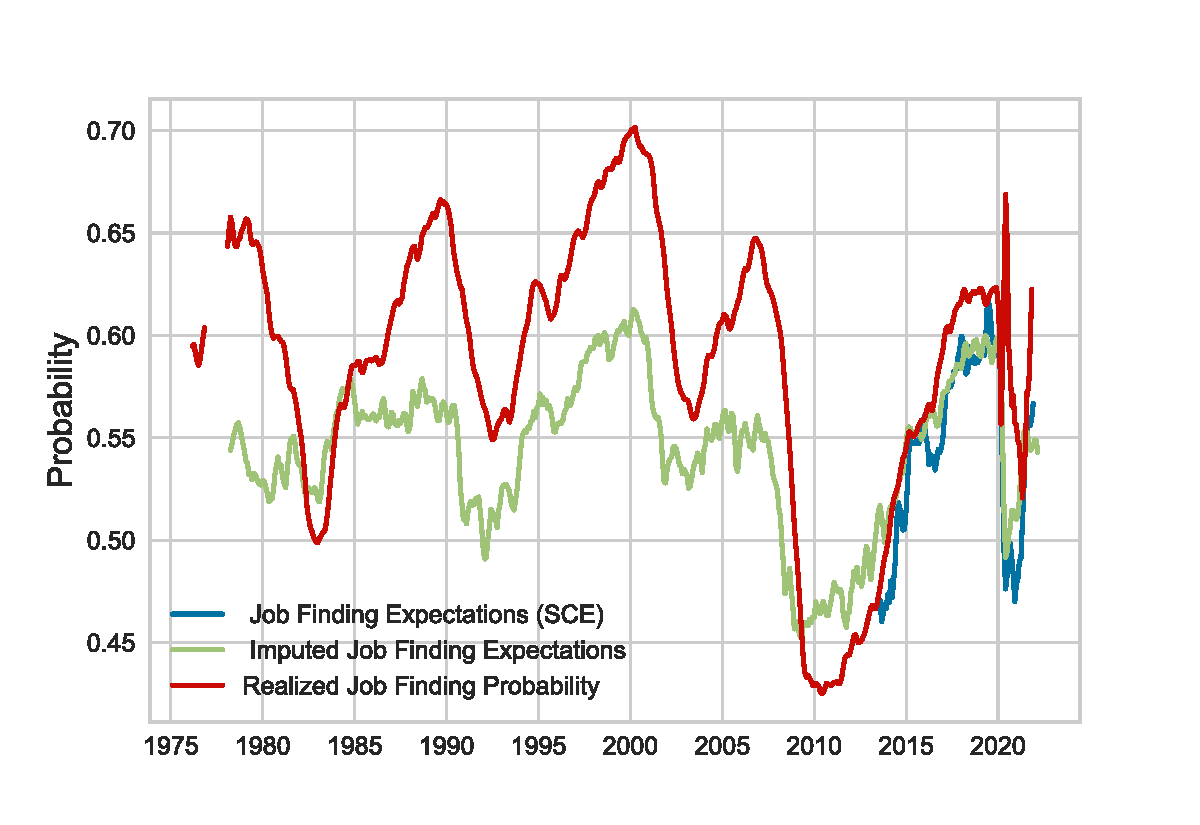
\includegraphics[scale=.75]{\FigDir/JF_imputation}
\end{figure} 

%%
%%\begin{figure}{}
   % \centering\includegraphics[scale=.26]{\FigDir/JS}
  %  \caption{Comparison of 5 month moving average of expectations of 1 year job separating probability against the actual 1 year job separating probability. }
%\end{figure}



%\begin{figure}{}
   % \centering\includegraphics[scale=.26]{\FigDir/JS2}
   % \caption{Comparison of raw expectations data of 1 year job separating probability, its 5 month moving average, and  the actual 1 year job separating probability. }
%\end{figure}
%%



%%More interestingly, in figure 2, a plot of the 5 month moving average of the  one year job separating expectations are presented against the realized one year job separating probability computed using \cite{shimer2012reassessing}'s method. For the series of actual job separation probabilities, I exclude observations during and after the pandemic because the job separation probabilities are derived from the job finding probabilities and thus many observations after the pandemic are missing. I focus on the correlation between both time series because I plan to have job separation expectations evolve according to a regression of the expectations on the realized values and likely their lags values as well.  Therefore the level difference between the time series will not matter as it will be captured by the intercept. Looking at the time series, beginning in early 2016, both series display a hump shape that rises and eventually falls back to its trend. For the expectations data, this hump lasts for at least a year while the the realized job separation data exhibits a much smaller hump that returns to its trend more quickly. This suggests that during this period, households were more pessimistic in the change in their probability of being fired compared to the actual data. In other words, households believed that the probability of losing a job had increased more than the actual job finding probability had increased. Overall, although the changes, or movements, in job finding probabilities does not seem to differ between expectations and the realized value, the job separation probabilities seem to display potential bias in updating beyond the level difference. This motivates endogenizing job separations as they may be the source of differences between a model of beliefs and its rational expectations counterpart.\\


\hypertarget{The-Model}{}
\section{The Model}

I present an heterogenous agents model with search and matching frictions, nominal rigidities, and beliefs on job finding probabilities.

\subsection{Households}
\label{subsec:Households}

There is a continuum of households of mass 1 distributed on the unit
interval and indexed by $i$. Households are ex-ante heterogeneous in their discount factors and subject to idiosyncratic income shocks and stochastic transition in their employment status. Households cannot observe the true job finding rate $\eta_{t}$ in period $t$ and instead hold the belief $\hat{\eta_{t}}$ of the job finding probability in period $t$. Each household solves  the following problem according to their \textit{perceived budget constraint}:

\begin{verbatimwrite}{\EqDir/supfn.tex}
\begin{eqnarray}
  \label{eq:supfn}
  \max_{\{\cLevBF_{it+s}\}_{s=0}^{\infty}} \mathrm{E_{t}}\left[\sum_{s=0}^{\infty} (\not D \beta^{t+s} U\left(  \cLevBF_{i t+s}, n_{i t+s}\right)\right]
\end{eqnarray}
\end{verbatimwrite}
\begin{eqnarray}
  \label{eq:supfn}
  \max_{\{\cLevBF_{it+s}\}_{s=0}^{\infty}} \mathrm{E_{t}}\left[\sum_{s=0}^{\infty} (\not D \beta_{i})^{t+s} U\left(  \cLevBF_{i t+s}, n_{i t+s}\right)\right]
\end{eqnarray}
 

subject to \\

Perceived Budget Constraint \\

\begin{align*}
\aLevBF_{it}     &= \mLevBF_{it} - \cLevBF_{it}   \label{eq:DBCparts} \\
\aLevBF_{it} +\cLevBF_{it}    &= \mathbf{z}_{it}(\hat{\eta_{t}}) +   (1 + r^{a}_{t} ) \aLevBF_{it-1} \\ 
\aLevBF_{it}  &\geq 0 \\
\end{align*}



The perceived budget constraint dictates the consumption policies to be solved while the true budget constraint below dictates the simulations of households in the model.\\

True Budget Constraint \\ 
\begin{align*}
\aLevBF_{it}     &= \mLevBF_{it} - \cLevBF_{it}    \\
\aLevBF_{it} +\cLevBF_{it}    &= \mathbf{z}_{it}(\eta_{t}) +   (1 + r^{a}_{t} ) \aLevBF_{it-1} \\ 
\aLevBF_{it}  &\geq 0 \\
\end{align*}




where
$U\left(\cLevBF_{i t}, n_{i t}\right) = \frac{\cLevBF_{i t}^{1-\rho}}{1 -\rho} - \varphi \frac{n_{it}^{1+v}}{1+v}$  and $\beta_{i}$ is the discount factor of household $i$. $\mLevBF_{it}$ \ denotes household $i$'s market resources at time $t$ to be expended on consumption or invested at a mutual fund. $\cLevBF_{it}$ is the level of consumption and $ \aLevBF_{it}$ is the value of household $i$'s shares at the mutual fund during period $t$ where the mutual fund's return is $r_{t+1}^{a}$.  $\mLevBF_{it}$ is determined by labor income,  $\mathbf{z}_{it}$, and the gross return on assets from the last period, $(1+r_{t}^{a}) \aLevBF_{it-1} $. $D$ is the probability of death. Death is included in our model to ensure permanent income, $\pLevBF$, and thus wealth, has a limiting distribution. The employment status of household $i$ at time $t$ is denoted by $n_{it}$ and follows a markov chain on the space $\{0,1\}$.  A household is employed when $n_{it} = 1$, otherwise he is unemployed. In particular,\\

\begin{align*} 
P(n_{it} = 1 | n_{it-1}) = \begin{cases}
       1 - \omega(1-\eta_{t}),   & \ n_{it-1} = 1 \\
       \eta_{t},  &  \ n_{it-1} = 0 \\
    \end{cases}\\
\end{align*}


\begin{align*} 
P(n_{it} = 0 | n_{it-1}) = \begin{cases}
        \omega(1-\eta_{t}),   & \ n_{it-1} = 1 \\
       1- \eta_{t},  &  \ n_{it-1} = 0 \\
    \end{cases}\\
\end{align*}

where  $\omega$ is the exogenous job separation rate. Households also believe their employment status follows the equation above with the important exception that they believe the job finding probability to be $\hat{\eta_{t}}$.\\


Labor income is subject to permanent and transitory idiosyncratic shocks. In particular, household $i$'s labor income is composed of a permanent component, $\pLevBF_{it} $ indicating the level of permanent income and a transitory component, $\tShkAll_{it} $, indicating the transitory income shock received by household $i$ at time $t$. $\pLevBF_{it} $ is subject to permanent income shocks $\pShk_{it+1}$ where $\pShk_{it}$ is iid mean one lognormal with standard deviation $\sigma_\pShk$, $\forall t$ . \\

\begin{align*}
\mathbf{z}_{it} &= \pLevBF_{it}\tShkAll_{it} \\
\pLevBF_{it+1} &=\pLevBF_{it} \pShk_{it+1} \\
\end{align*}


The transitory component follows   \\


\begin{align*}
\tShkAll _{it}=  (1-\tau_{t})\tShkEmp_{it} w_{t} n_{it} + u ( 1 - n_{it} )
\end{align*}




where u are unemployment benefits, $w_{t}$ is the real wage, and $\tShkEmp_{t}$ is an iid mean-one lognormal with standard deviation $\sigma_{\tShkEmp}$.  



\hypertarget{Beliefs}{}
\subsection{Beliefs}

\label{subsec: Beliefs}

Beliefs over the job finding probabilities $\hat{\eta_{t}}$ are updated following:

$$\hat{\eta_{t}} =  \beta_{\eta} \eta  + \epsilon_{\eta_{t}}$$ \\


where $\beta_{\eta}$ is the job finding belief reaction coefficient and captures the reaction of households. 

Let  $\epsilon_{\eta_{t+1}} = \rho_{ \eta} \epsilon_{{\eta}_{t} }+ v_{\eta}$.

\begin{comment}
Combining the transition equations, the recursive nature of
the problem allows us to rewrite it more compactly in Bellman equation form,
\begin{eqnarray*}
\VFunc_{t}(\mLevBF_{t},\pLevBF_{t}) & = & \max_{\cLevBF_{t}}~\left\{\util(\cLevBF_{t})+\DiscFac \Ex_{t}\left[ \VFunc_{t+1}((\mLevBF_{t}-\cLevBF_{t})\Rfree+ \pLevBF_{t+1}\tShkAll_{t+1},\pLevBF_{t} \PGro  \pShk_{t+1})\right]\right\}
.
\end{eqnarray*}
\end{comment} 

\hypertarget{Financial Intermediary}{}
\subsection{Financial Intermediary}

\label{subsec:Financial Intermediary}

The financial intermediary performs a mutual fund activity where it collects assets from households and invests them into stocks $v_{jt}$, and nominal reserves $M_{t}$ at the central bank.\\ 

In particular, at the end of period $t$, the assets collected from households $A_{t}$ must be invested into shares $\mathit{v}_{jt}$ of firm $j$ at price  $q^{s}_{jt}$,  and nominal reserves $M_{t}$. 

\begin{equation} A_{t} =  \int_{0}^{1} q^{s}_{jt}\mathit{v}_{jt}\,dj  + \frac{M_{t}}{P_{t}}\end{equation}

where $A_{t} $ is the dollar value of the mutual fund's assets at the end of period $t$ and $ \mathit{v}_{jt}$ is the portfolio share of firm $j$ stocks with $\int_{0}^{1} \mathit{v}_{jt}\,dj =1$.  \\

The mutual fund's return in the next period is then 

$$(1+r^{a}_{t+1})  = \frac{  \int_{0}^{1} (q^{s}_{jt+1}+ D_{jt+1})\mathit{v}_{jt} \, dj +(1+i_{t}) \frac{M_{t}}{P_{t+1}}}{A_{t}}$$\\ 

where  $D_{jt+1}$ are dividends of firm $j$ and $i_{t}$ is the nominal interest rate  on nominal reserves. \\ \\

The mutual fund is risk neutral and looks to maximize its expected return 

$$\max_{ M_{t} , \mathit{v}_{jt} \}} \mathrm{E}_{t}\left[1+r^{a}_{t+1} \right] = \mathrm{E}\left[ \frac{ \int_{0}^{1} (q^{s}_{jt+1}+ D_{jt+1})\mathit{v}_{jt} \, dj +(1+i_{t}) \frac{M_{t}}{P_{t+1}}}{\frac{M_{t}}{P_{t}}  + \int_{0}^{1} q^{s}_{jt}\mathit{v}_{jt}\,dj} \right]$$ \\

 
The first order conditions lead to the no arbitrage equations:

\begin{equation} \mathrm{E}_{t}\left[1+r^{a}_{t+1}\right] =\frac{\mathrm{E}_{t}\left[q^{s}_{jt+1} + D_{jt+1} \right]}{q^{s}_{jt}} = (1+i_{t}) \mathrm{E}_{t}\left[\frac{P_{t}}{P_{t+1}}\right] \equiv 1 +r_{t} \end{equation}

where $r_{t}$ is defined to be the real interest rate in period $t$. 
In equilibrium ,we will assume $M_{t} =0$ \\ \\

\hypertarget{Goods Market}{}
\subsection{Goods Market}

There is a continuum of  monopolistically competitive intermediate good producers indexed by $j \in [0,1]$ who produce intermediate goods $Y_{jt}$ to be sold to a final good producer at price $P_{jt}$. Using intermediate goods $Y_{jt}$ for $j \in [0,1]$, the  final good producer produces a final good $Y_{t}$ to be sold to households at price $P_{t}$.  \\ 


\hypertarget{Final Good Producer}{}
\subsubsection{Final Good Producer}

A perfectly competitive final good producer purchases intermediate goods $Y_{jt}$ from intermediate good producers at price $P_{jt}$ and produces a final good $Y_{t}$ according to a CES production Function. 

$$ Y_{t} = \left(\int_{0}^{1} Y_{jt}^{\frac{\epsilon_{p}-1}{\epsilon_{p}}}\, dj\right)^{\frac{\epsilon_{p}}{\epsilon_{p}-1}}$$ \\

where $\epsilon_{p}$ is the elasticity of substitution. \\ 

Given $P_{jt}$ , the price of intermediate good $j$ ,  the final good producer maximizes his profit

$$ \max_{Y_{jt}} P_{t} \left(\int_{0}^{1} Y_{jt}^{\frac{\epsilon_{p}-1}{\epsilon_{p}}}\, dj\right)^{\frac{\epsilon_{p}}{\epsilon_{p}-1}} - \int_{0}^{1} P_{jt} Y_{jt} ,\ dj $$ \\


The first order condition leads to demand for good $j$

\begin{equation} Y_{jt} = \left(\frac {P_{jt}}{P_{t}}\right)^{- \epsilon_{p}} Y_{t}\end{equation} \\

and the price index

\begin{equation} P_{t} = \left(\int_{0}^{1} P_{jt}^{1-\epsilon_{p}}\,dj \right )^{\frac{1}{1-\epsilon_{p}}} \end{equation}


\hypertarget{Intermediate Good Producer}{}
\subsubsection{Intermediate Good Producer}

Intermediate goods producers employ labor and produce according to a Cobb Douglas Production function. 

$$Y_{jt} =  Z_{t}  N_{jt}$$ 

where $log(Z_{t}) = \rho_{Z} log( Z_{t-1}) + \epsilon_{Z}$ \\ \\

  
 
 Firm $j$ chooses $P_{jt}$ to maximize its dividend $D_{jt}$ and its stock price $q^{s}_{jt} $ facing price stickiness a la \cite{rotemberg1982sticky}.
 
  
  $$\max_{\{P_{jt}\}} \overbrace{\frac{P_{jt}Y_{jt}}{P_{t}} - w_{t} N_{jt} - \kappa v_{jt} -  \frac{\varphi}{2}\left( \frac{P_{jt} - P_{jt-1}}{P_{jt-1}} \right)^{2} Y_{t} }^{ \equiv D_{jt}} + q^{s}_{jt}\left(P_{jt}\right) $$

  
Given $q^{s}_{jt}\left(P_{jt}\right) = \frac{\mathrm{E}_{t}\left[q^{s}_{jt+1} + D_{jt+1}\left(P_{jt}\right)\right]}{1+r_{t}}$,  this is equivalent to: 
 
 $$\max_{\{P_{jt}\}} \mathrm{E}_{t}\left[\sum_{s=0}^{\infty}  M_{t,t+s}D_{jt+s} \right]$$
 
subject to $$Y_{jt} = \left(\frac {P_{jt}}{P_{t}}\right)^{- \epsilon_{p}} Y_{t}$$

$$ N_{jt} =  \frac{Y_{jt}} {Z_{t}} $$ 


$$ v_{jt} =  \frac{ N_{jt} - (1-\omega)N_{jt-1}}{\phi_{t}} $$

$$ v_{jt} \geq 0$$
 
where $M_{t, t+s-1} = \prod_{k=t}^{t+s} \frac{1}{1+r_{k}}$ is the stochastic discount factor. \\

The problem can be rewritten as 

$$\max_{\{P_{jt}\}} \mathrm{E}_{t}\left[\sum_{s=0}^{\infty}  M_{t,t+s} \left( \left( \frac{P_{jt+s}}{P_{t+s}} - MC_{t+s}\right)Y_{jt+s} -  \frac{\varphi}{2}\left( \frac{P_{jt+s}}{P_{jt+s-1}} - 1\right)^{2} Y_{t+s} \right)\right]$$


where $MC_{t} = \frac{1}{Z_{t}} \left( w_{t} + \frac{\kappa}{\phi_{t}} - \lambda_{t} - M_{t,t+1} (1-\omega) \left[  \frac{\kappa}{\phi_{t+1}} - \lambda_{t+1} \right] \right)$ \\



Firms can change their price in each period, subject to the payment of the adjustment cost.
Hence, all the firms face the same problem, and thus will choose the same price, producing the same quantity. In other words $P_{jt} =P_{t}$ and $Y_{jt} =Y_{t}$.\\ 

The resulting Phillips Curve is defined by


$$ \epsilon_{p} MC_{t} = \epsilon_{p} - 1 + \varphi ( \Pi_{t} -1) \Pi_{t} - M_{t,t+1} ( \varphi (\Pi_{t+1} -1 ) \Pi_{t+1} \frac{Y_{t+1}}{Y_{t}}$$

where $ \Pi_{t} = \frac{P_{t}}{P_{t+1}}$.



\hypertarget{Labor Market}{}
\subsection{Labor Market}

Every period a proportion $\omega$ of workers lose their job, and firm j post vacancies $v_{jt}$. Each vacancy is filled with probability $\phi_{t}$. Assuming firms are very large so that a large number of vacancies are posted, the level of filled vacancies is $v_{jt}\phi_{t}$ for firm j.

$$ N_{jt} = (1-\omega)N_{jt-1} + v_{jt} \phi_{t}$$

Workers search for jobs:

$$m_{t} = \chi e_{t}^{\alpha} v_{t}^{1-\alpha}$$

$m_{t}$ is the number of matches in period $t$.\\

Then define $\eta_{t}$ to be the job finding probability and $\phi_{t}$ the vacancy filling rate:

$$ \eta_{t} = \frac{m_{t}}{e_{t}} = \chi \Theta_{t}^{1-\alpha}$$

$$ \phi_{t} = \frac{m_{t}}{v_{t}} = \chi \Theta_{t}^{-\alpha} = \eta_{t}^{\frac{\alpha}{\alpha -1}} \chi^{\frac{-1}{\alpha - 1}}$$

Aggregating $N_{jt}$ across $j$ we have the law of motion for labor:

$$ N_{t} =  (1-\omega)N_{t-1} + m_{t} $$

$$ e_{t} = 1 - (1-\omega) N_{t-1} $$


\hypertarget{Wage Determination}{}
\subsection{Wage Determination }


Following \cite{broer2021unemployment}, I assume the real wage to be fixed.

$$ w_{t} = w_{ss}$$

As \cite{broer2021unemployment} notes, recent research has documented nominal wage rigidities to be pervasive in the US labor market. Given the shocks I study are contractionary and that the response of inflation in my model to contractionary shocks to be procyclical, this is likely a weak assumption. Further, a fixed real wage reduces the computational complexity of the model as wage bargaining with a distribution of households is not trivial to implement. 


\hypertarget{Government}{}
\subsection{Government}

\hypertarget{Fiscal Policy}{}
\subsubsection{Fiscal Policy}

I follow \cite{Kekre2021} and \cite{challe2017precautionary} by having the government tax labor income from employed households to fund unemployment insurance for the unemployed.

$$ u(1 -N_{t}) = \tau_{t} w_{t}N_{t}$$

\hypertarget{Monetary Policy}{}
\subsubsection{Monetary Policy}


The central bank follows the taylor rule: 

$$i_{t} = r^{*} +\phi_{\pi} \pi_{t}  + \epsilon^{m}_{t}$$ \\

where $\phi_{\pi}$ is the Taylor rule coefficient for inflation,  $r^{*}$ is the steady state interest rate, $Y_{ss}$ is the steady state level of output,  $\epsilon^{m}_{t} = \rho_{v} \epsilon^{m}_{t-1} +\varepsilon_{t}$ are innovations to the taylor rule. \\

\hypertarget{Equilibrium}{}
\subsection{Equilibrium}


An equilibrium in this economy is a sequence of: \\

- Policy Functions $\left( c_{it}(m) \right )_{t=0}^{\infty}$ \\

- Prices $ \left(r_{t},  r^{a}_{t+1}, i_{t}, q^{s}_{t},  w_{t} , \pi_{t} , \tau_{t} \right) _{t=0}^{\infty}$\\

- Aggregates $ \left(C_{t}, Y_{t} , N_{t}, \hat{\eta_{t}},\eta_{t}, \phi_{t}, v_{t},  D_{t} , A_{t}  \right)_{t=0}^{\infty}$\\

Such that: \\

$ \left(  c_{it}(m)\right)_{t=0}^{\infty}$  solves the household's maximization problem given $  \left( w_{t}, \hat{\eta_{t}},  r^{a}_{t} \right)_{t=0}^{\infty}$.\\

The Mutual fund, final goods producer, intermediate goods producers maximize their objective function. \\

The nominal interest rate is set according to the central bank's Taylor rule. \\

The tax rate is determined by the government budget constraint. \\

Markets clear:

 $$ A_t =  q^{s}_{t} =  \int_{0}^{1} \pLevBF_{it}\left( m_{it} - c_{it}(m_{it})\right) \, di $$\\
 
$$ C_{t} =w_{t}N_{t} + D_{t}   $$\\

 
 where $C_{t} \equiv  \int_{0}^{1} \pLevBF_{it} c_{it}(m_{it})\, di $ \\



\hypertarget{Calibration }{}
\section{Calibration }

Table 1 and 2 summarize the calibration of the model. The model is calibrated to a quarterly frequency. 


\hypertarget{Households }{}
\subsection{Households }

I set the CRRA to equal a standard value of 2. I follow \cite{carroll2017distribution} and let the standard deviation of permanent shocks to be .06 and the standard deviation of transitory shocks to be .2 . To target a 40 year work life, the probability of death is set to 1 - .99735. The tax rate is set to .18 and the real wage is 2.0.  The unemployment replacement rate is set to 35\% of the real wage . Although the typical replacement rate across states in the US is around 50\%,  the majority of the unemployed do not receive unemployment benefits( \cite{Graves2022}, \cite{CRLK2016}). The job separation rate is set to .1 in line with \cite{Graves2022} and \cite{Kekre2021} and the job finding probability is .667 to target a 5\% steady state unemployment rate and a 1.5 quarter duration of unemployment.  The steady state real interest rate is set to 3\% per annum and the resulting discount factor is internally calibrated to reach an employed MPC of .46, consistent with the findings of \cite{Kekre2021}. The job finding belief reaction coefficient is calibrated to .6, in the upper range of estimates reported by Du, Qiu, and Wang (2022).  \\

\begin{table}
\begin{center}\renewcommand{\arraystretch}{1.5}
\caption{Household Calibration}\label{table:Calibration}
\begin{tabular}{|c|ccl|c|}
\hline
\multicolumn{5}{|l|}{Calibrated Parameters}  \\ \hline
Description                     & \multicolumn{1}{c}{Parameter} & Value & \multicolumn{2}{c|}{Source/Target }\\ \hline
CRRA & \multicolumn{1}{c}{$\CRRA$} & 2 & \multicolumn{2}{c|}{Standard} \\
Belief Reaction Coefficient   & \multicolumn{1}{c}{$\beta_{\eta}$} & .6 & \multicolumn{2}{c|}{Du, Qiu, and Wang (2022) } \\
Real Interest Rate                 & \multicolumn{1}{c}{$r$} & $1.03^{.25} - 1$ & \multicolumn{2}{c|}{ 3\% annualized real rate} \\
Discount Factor          & \multicolumn{1}{c}{$\beta$} & 0.961 & \multicolumn{2}{c|}{Employed MPC = 0.47 } \\
Probability of Death       & \multicolumn{1}{c}{$\not D$} & 0.00625 & \multicolumn{2}{c|}{40 Year Work Life} \\
Tax Rate       & \multicolumn{1}{c}{$\tau$} & 0.18 & \multicolumn{2}{c|}{} \\
Real Wage & \multicolumn{1}{c}{$w$} & 2.0 & \multicolumn{2}{c|}{} \\
Unemployment Benefits & \multicolumn{1}{c}{$u$} & 0.7 & \multicolumn{2}{c|}{ 35\% Replacement Rate} \\
Job Finding Rate & \multicolumn{1}{c}{$\eta$} & 0.667 & \multicolumn{2}{c|}{ 5\% Unemployment Rate} \\
Job Separation Rate & \multicolumn{1}{c}{$\omega$} & 0.1 & \multicolumn{2}{c|}{\cite{Graves2022}} \\
Std Dev of Log Permanent Shock  & \multicolumn{1}{c}{$\sigma_{\pshk}$} & 0.06 & \multicolumn{2}{c|}{Carroll et al. (2017)} \\
Std Dev of Log Transitory Shock & \multicolumn{1}{c}{$\sigma_{\theta}$} & 0.2 & \multicolumn{2}{c|}{Carroll et al. (2017)} \\ \hline
\end{tabular}
\end{center}
\end{table}
\begin{table}
\begin{center}\renewcommand{\arraystretch}{1.5}
\caption{Economy Calibration}\label{table:Calibration}
\begin{tabular}{|c|ccl|c|}
\hline
\multicolumn{5}{|l|}{Calibrated Parameters}  \\ \hline
Description                     & \multicolumn{1}{c}{Parameter} & Value & \multicolumn{2}{c|}{Source/Target }\\ \hline
Elasticity of Substitution       & \multicolumn{1}{c}{$\epsilon_{p}$} & 310 & \multicolumn{2}{c|}{$\beta = 0.961$ } \\
Price Adjustment Costs & \multicolumn{1}{c}{$\varphi$} & 3100 & \multicolumn{2}{c|}{Slope of Phillips Curve = .1} \\
Vacancy Filling Rate & \multicolumn{1}{c}{$\phi$} & 0.71 & \multicolumn{2}{c|}{Wouter et al. (2000)} \\
Matching Elasticity & \multicolumn{1}{c}{$\alpha$} & 0.72 & \multicolumn{2}{c|}{\cite{SilvaToledo}} \\
Vacancy Cost & \multicolumn{1}{c}{$\kappa$} & 0.156 & \multicolumn{2}{c|}{7.8\% of Real Wage} \\
 Government Spending       & \multicolumn{1}{c}{$G$} & 0.30 & \multicolumn{2}{c|}{} \\
Taylor Rule Inflation Coefficient        & \multicolumn{1}{c}{$\phi_{\pi}$} & 1.5 & \multicolumn{2}{c|}{Standard} \\
Liquid Assets to Output Ratio       & \multicolumn{1}{c}{$\frac{A}{Y}$} & .44 & \multicolumn{2}{c|}{} \\
Persistence of Monetary Policy Shock      & \multicolumn{1}{c}{$\rho_{v}$} & .85 & \multicolumn{2}{c|}{Graves (2022)} \\ \hline
\end{tabular}
\end{center}
\end{table}


\hypertarget{Rest of the Economy }{}
\subsection{Rest of the Economy }

The quarterly vacancy filling rate is .71 as in \cite{Wouter2000}. The matching elasticity is .72 following \cite{SilvaToledo} and the vacancy cost is set to 7.8\% of the real wage, near the 7\% target calibrated in \cite{Christiano2016} and within the range of plausible values of this statistic reported by \cite{SilvaToledo}\footnote{The range of plausible values lie between 4\% and 14\%}. The elasticity of substitution is set to 310 to target the discount factor value of .961. This assumption is required to clear the asset market clearing condition found at the end of section 4.8. Asset supply in this model is a function of dividends earned by firms and thus a large markup is incompatible with a low level of asset demand generated form a smaller discount factor. In addition, this assumption is almost equivalent to having firms receive zero profits in equilibrium and does not affect the results below. If anything, having zero profits attenuates the amplification mechanism as households do not receive profits. In \cite{Kekre2021} he assumes a elasticity of substitution of 6 although when calibrating his model to the distribution of liquid assets, assumes firms face a tax rate to lead to earn no profits in equilibrium. Instead of adding a tax rate to firms, I simply assume a large elasticity of substitution to ensure near zero proftis to allow my asset market to clear. The price adjusment cost parameter is set to 3100 to target phillips curve slope of .1. With a tax rate of .18,  Government Spending is set to .3 to clear the government budget constraint and the discount factor of .961 implies a liquid assets to output ratio of .44.  The job finding belief reaction coefficient is calibrated to .6, in the upper range of estimates reported by Du, Qiu, and Wang (2022).



\hypertarget{Model Validation }{}
\subsection{Model Validation }

In this section, I give confidence to the calibration of households by verifying that my model is consistent with some key empirical moments documented in the microdata on household consumption. In particular, I verify that the model is consistent with the empirical dynamic consumption response to income shocks and the MPCs of the employed and unemployed documented in the microdata.  \\

\begin{figure}
    \centering
     \caption{Comparison of Model IMPCs vs Data from Fagereng et al. (2021)}
    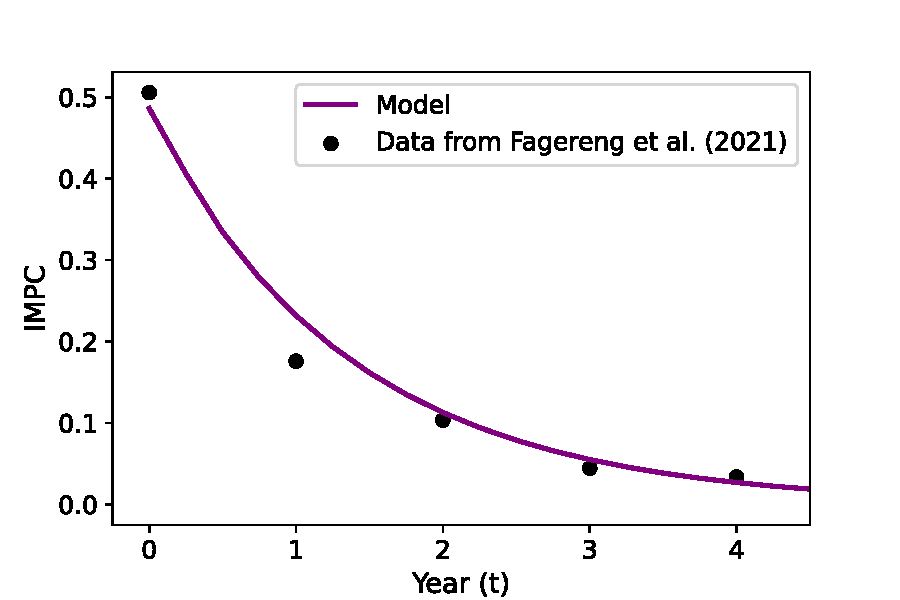
\includegraphics[scale=.8]{\FigDir/Model_vs_Fagereng}
    \floatfoot{This figure plots the IMPCs produced by the model against the IMPCs found from the data in Fagereng et al.(2021). The IMPCs of the model are computed by simulating an unanticipated one time transitory shock to income in period 0. Then the IMPC is computed as $IMPC_{t} = \frac{dC_{t}}{dZ_{0}} $  where $dC_{t}$ is the change in consumption relative to the steady state in period $t$, and $dZ_{0}$ is the size of the income shock.}
    \label{fig:IMPCs}
\end{figure}

Figure \ref{fig:IMPCs} demonstrates the intertemporal MPCs\footnote{The intertemporal MPCs, or IMPCs, is defined as the consumption response in t + j to a transitory income shock in period t, where $j \geq 0$. Intuitively, it is the consumption response tomorrow (or today) to a transitory income shock today. \cite{Fagereng2021} use Norwegian administrative data to estimate the dynamic consumption responses to income shocks. } of the model are consistent with the estimates from \cite{Fagereng2021}. This implies the model nearly captures the empirical dynamic response of consumption to income shocks. In year 0, the empirical estimate for the MPC is .5 while the model produces an MPC of .485 while in year 0 the empirical estimate is .176, .056 less than its model counterpart. Still, the overall timepath of the consumption response is consistent with \cite{Fagereng2021} and vital to the general equilibrium transmission of shocks in models with heterogeneous agents and nominal rigidities (\cite{auclert2018intertemporal}). \\
 
 

Table 3 demonstrates the model matches the annual MPC out of unexpected, transitory income shocks of both the employed and unemployed documented by \cite{Kekre2021} \footnote{\cite{Kekre2021} uses the 2010 Survey of Household Income and Wealth to estimate the sample mean of the self reported MPCs.} . These are important moments to match as employed households are taxed to fund unemployment benefits. Thus, a shock that leads to changes in the unemployment rate will produce an empirically consistent consumption response to both changes in taxes for the employed and increases in UI receipts for the unemployed. \\


 \begin{table}
\begin{center}\renewcommand{\arraystretch}{1.5}
\caption{Moments}\label{table:Calibration}
\begin{tabular}{|c|ccl|c|}
\hline

Moment                     & \multicolumn{1}{c}{Estimate} & Source & \multicolumn{2}{c|}{Model }\\ \hline
Employed MPC - Unemployed MPC (Annual) & \multicolumn{1}{c}{.25} & \cite{Kekre2021} & \multicolumn{2}{c|}{.24} \\ \hline
Employed MPC  (Annual) & \multicolumn{1}{c}{.47} & \cite{Kekre2021} & \multicolumn{2}{c|}{.47} \\ \hline
Unemployed MPC  (Annual) & \multicolumn{1}{c}{.72} & \cite{Kekre2021} & \multicolumn{2}{c|}{.71} \\ \hline
\end{tabular}
\end{center}
\end{table}
 


\hypertarget{ Impulse Response to a Monetary Policy Contraction}{}
\section{Impulse Response to a Monetary Policy Contraction }


In this section, I study how underreaction in job finding expectations influence fluctuations due to a monetary policy shock.  Figure \ref{fig:IPR_ev} illustrates the impulse responses to a 10bp (annualized) shock to the nominal interest rate with persistence .85 under two different model calibrations. I compare a model with rational households ( $\beta_{\eta} = 1$) against a model with underreactive households ($\beta_{\eta} = .6$) to illustrate the effects of underreactive beliefs. \\

\begin{figure}{}
    \centering
        \caption{Impulse Responses to Monetary Contraction Shock }
        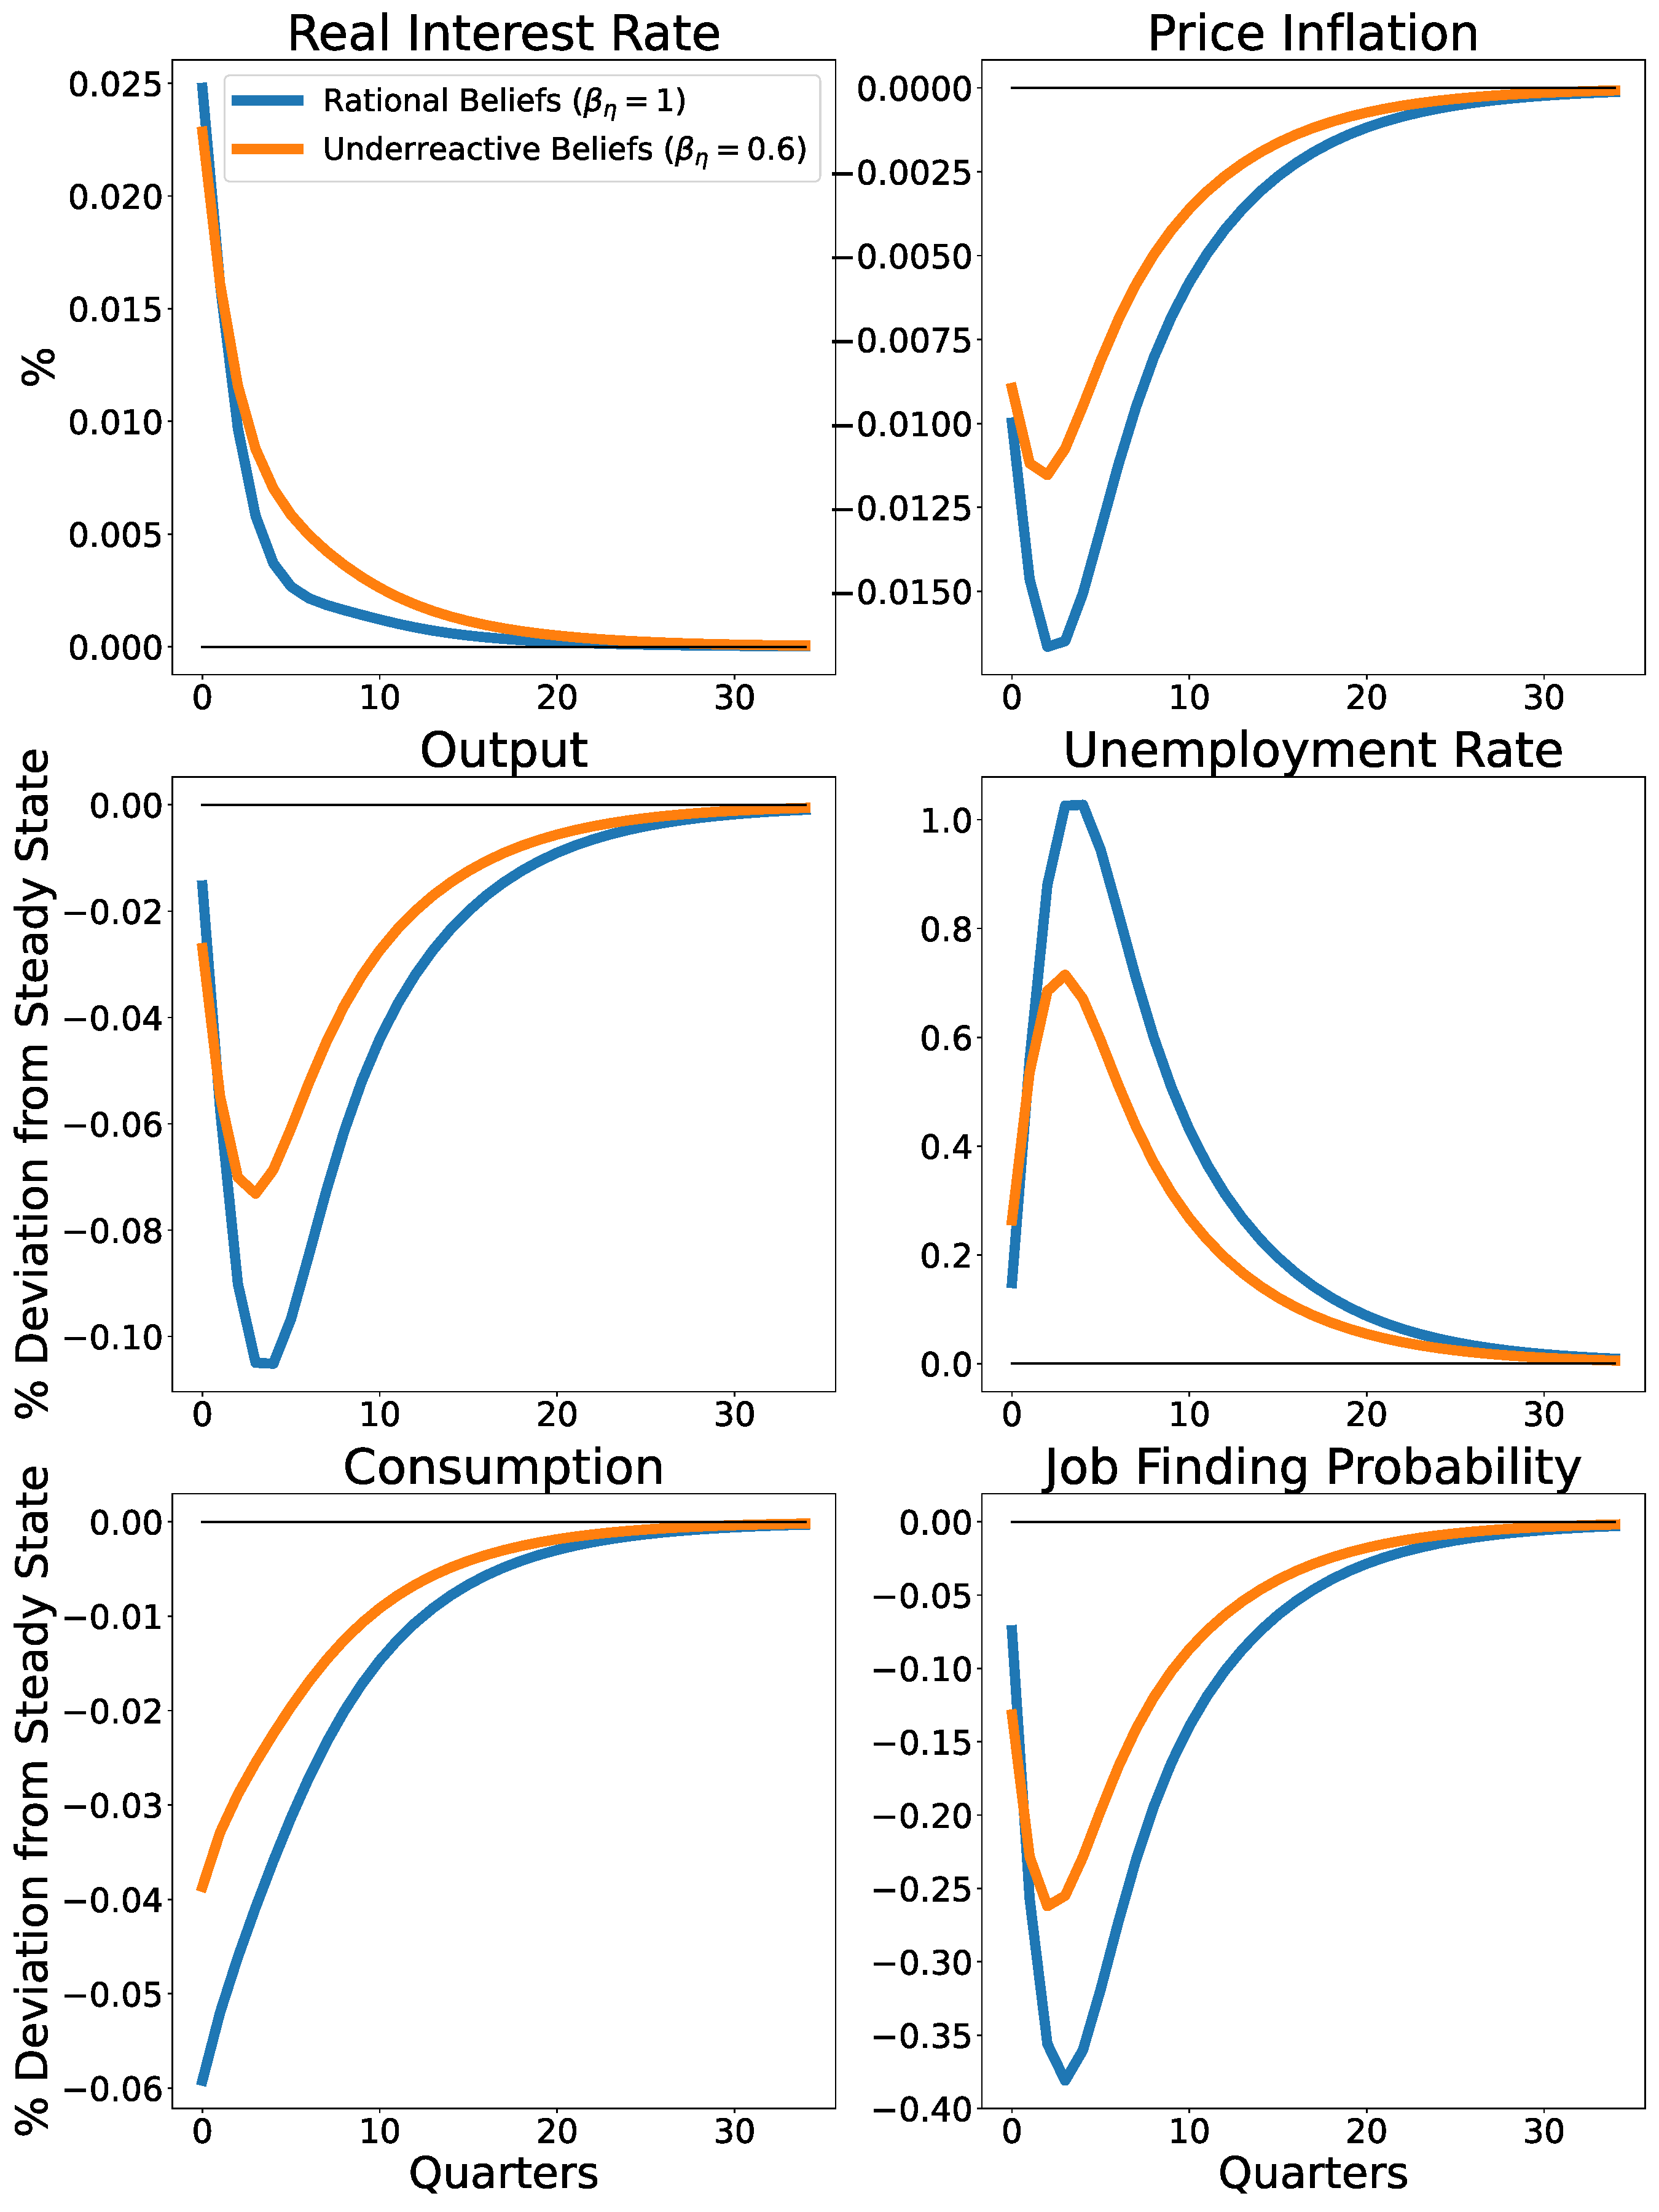
\includegraphics[scale=.3]{\FigDir/ev_shock_comparison_basic}
     \label{fig:IPR_ev}
\end{figure}


The impulse responses to the model with underreactive beliefs are attenuated compared to the model with rational households (model with $\beta_{\eta}=1$).  In both calibrations of the model, a rise in the nominal rate raises the real interest rate causing downward pressure on aggregate consumption due to the intertemporal substitution channel. Given that output is demand determined, output and labor must fall decreasing labor tightness and the job finding probability. The fall in the job finding probability raises the probability of being unemployed and induces households to increase their precautionary savings. This rise in precautionary savings leads consumption to decline further and as a consequence amplifies the business cycle. Because the households in the model with underreactive model do not perceive their unemployment risk to rise as substantially in comparison to the baseline HANK and SAM, the rise in precautionary saving is dampened and therefore the amplification of the business cycle is attenuated.\\

This attenutation exhibits the effects of underreactive beliefs on aggregate demand. The supply side of effects of underreactive job finding expectations may reverse the attenuation of the impulse responses. Notably, the inclusion of wage bargaining may amplify the impulse responses of the underreactive model as stubborn job finding beliefs will induce wage stickiness (\cite{menzio2022stubborn}). \\
%As a consequence, the results above demonstrate the effects of underreactive beliefs on aggregate demand. \\

\hypertarget{ Quantifying The Precautionary Channel}{}
\section{Quantifying The Precautionary Channel}

In this section, I quantify the precautionary channel to a monetary policy contraction. I find the precautionary channel to explain a significant share of the volatility in fluctuations following a monetary policy shock.


\hypertarget{Magnitude of The Precautionary Channel}{}
\subsection{Magnitude of The Precautionary Channel}

To quantify the precautionary channel, I compute the share of the variance of the responses of consumption and the unemployment due to precautionary saving. \\ 

\begin{figure}
    \centering
    
        \caption{Impulse Responses to Monetary Contraction Shock (Precautionary Channel)}
    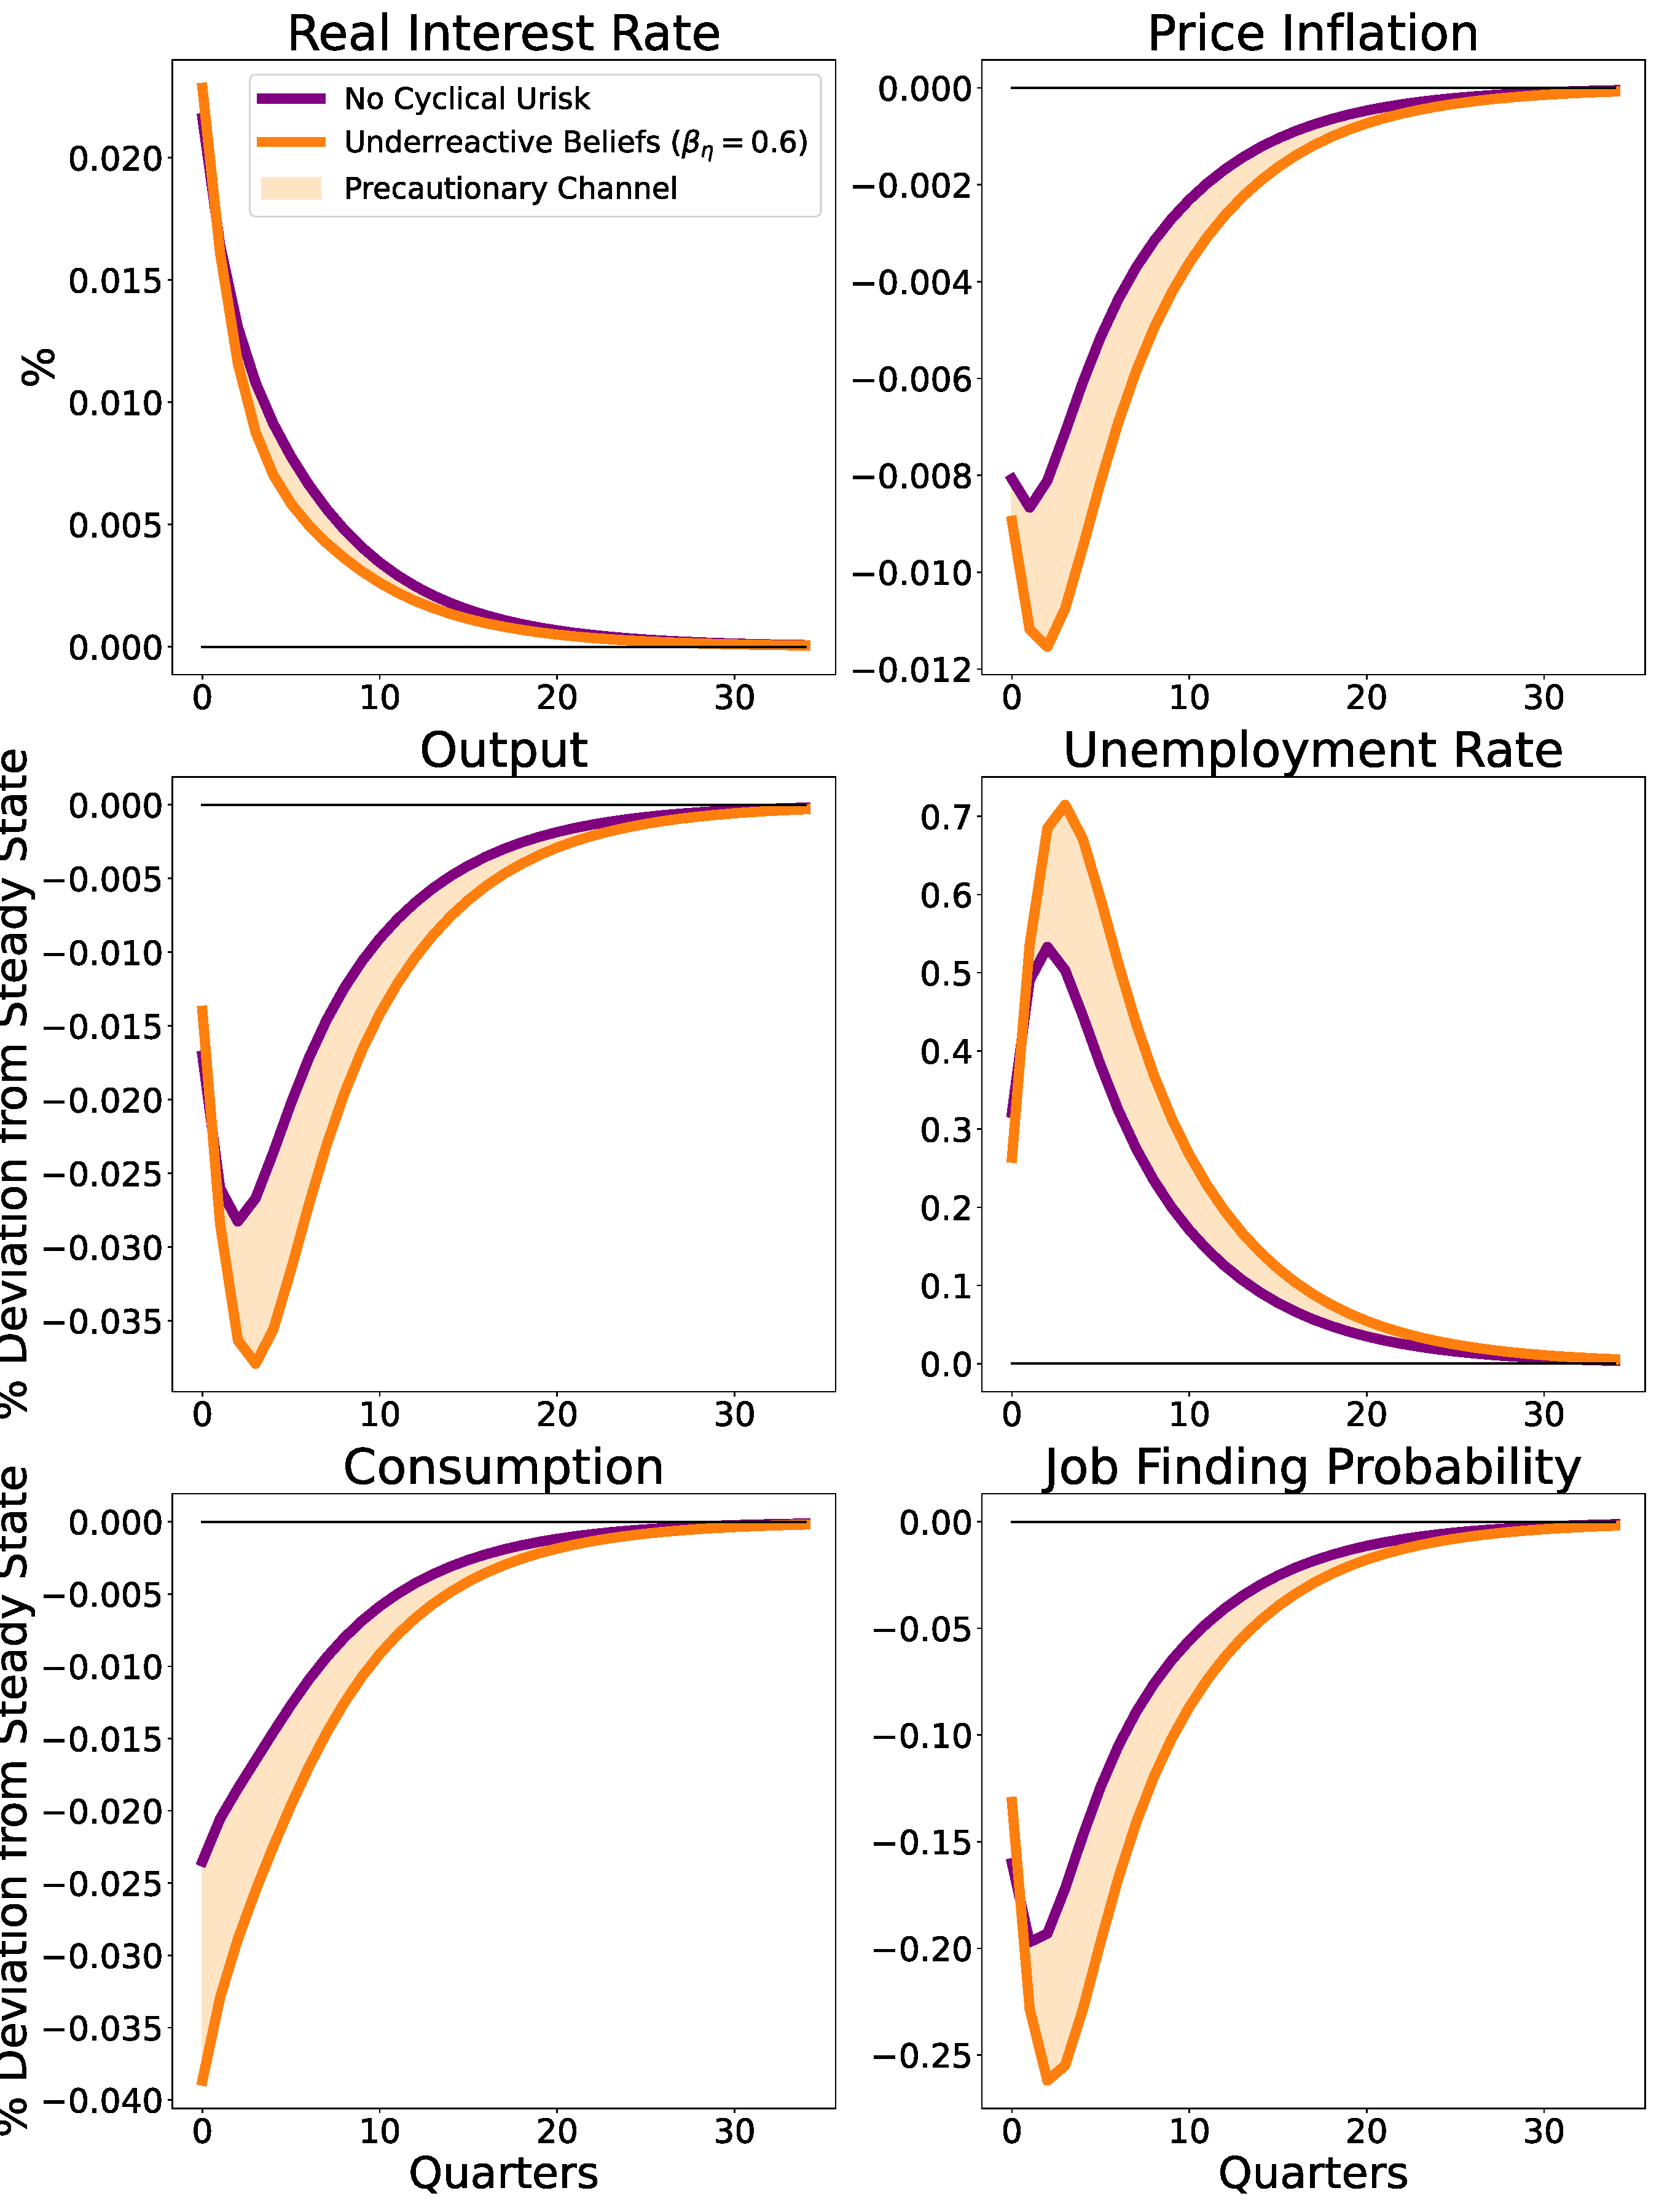
\includegraphics[scale=.3]{\FigDir/ev_shock_comparison_Urisk}

     \label{fig:IPR_ev_Urisk}
\end{figure}



%\begin{figure}
%    \centering
%      \caption{Impulse Responses to Consumption and Unemployment (Precautionary Channel)}
%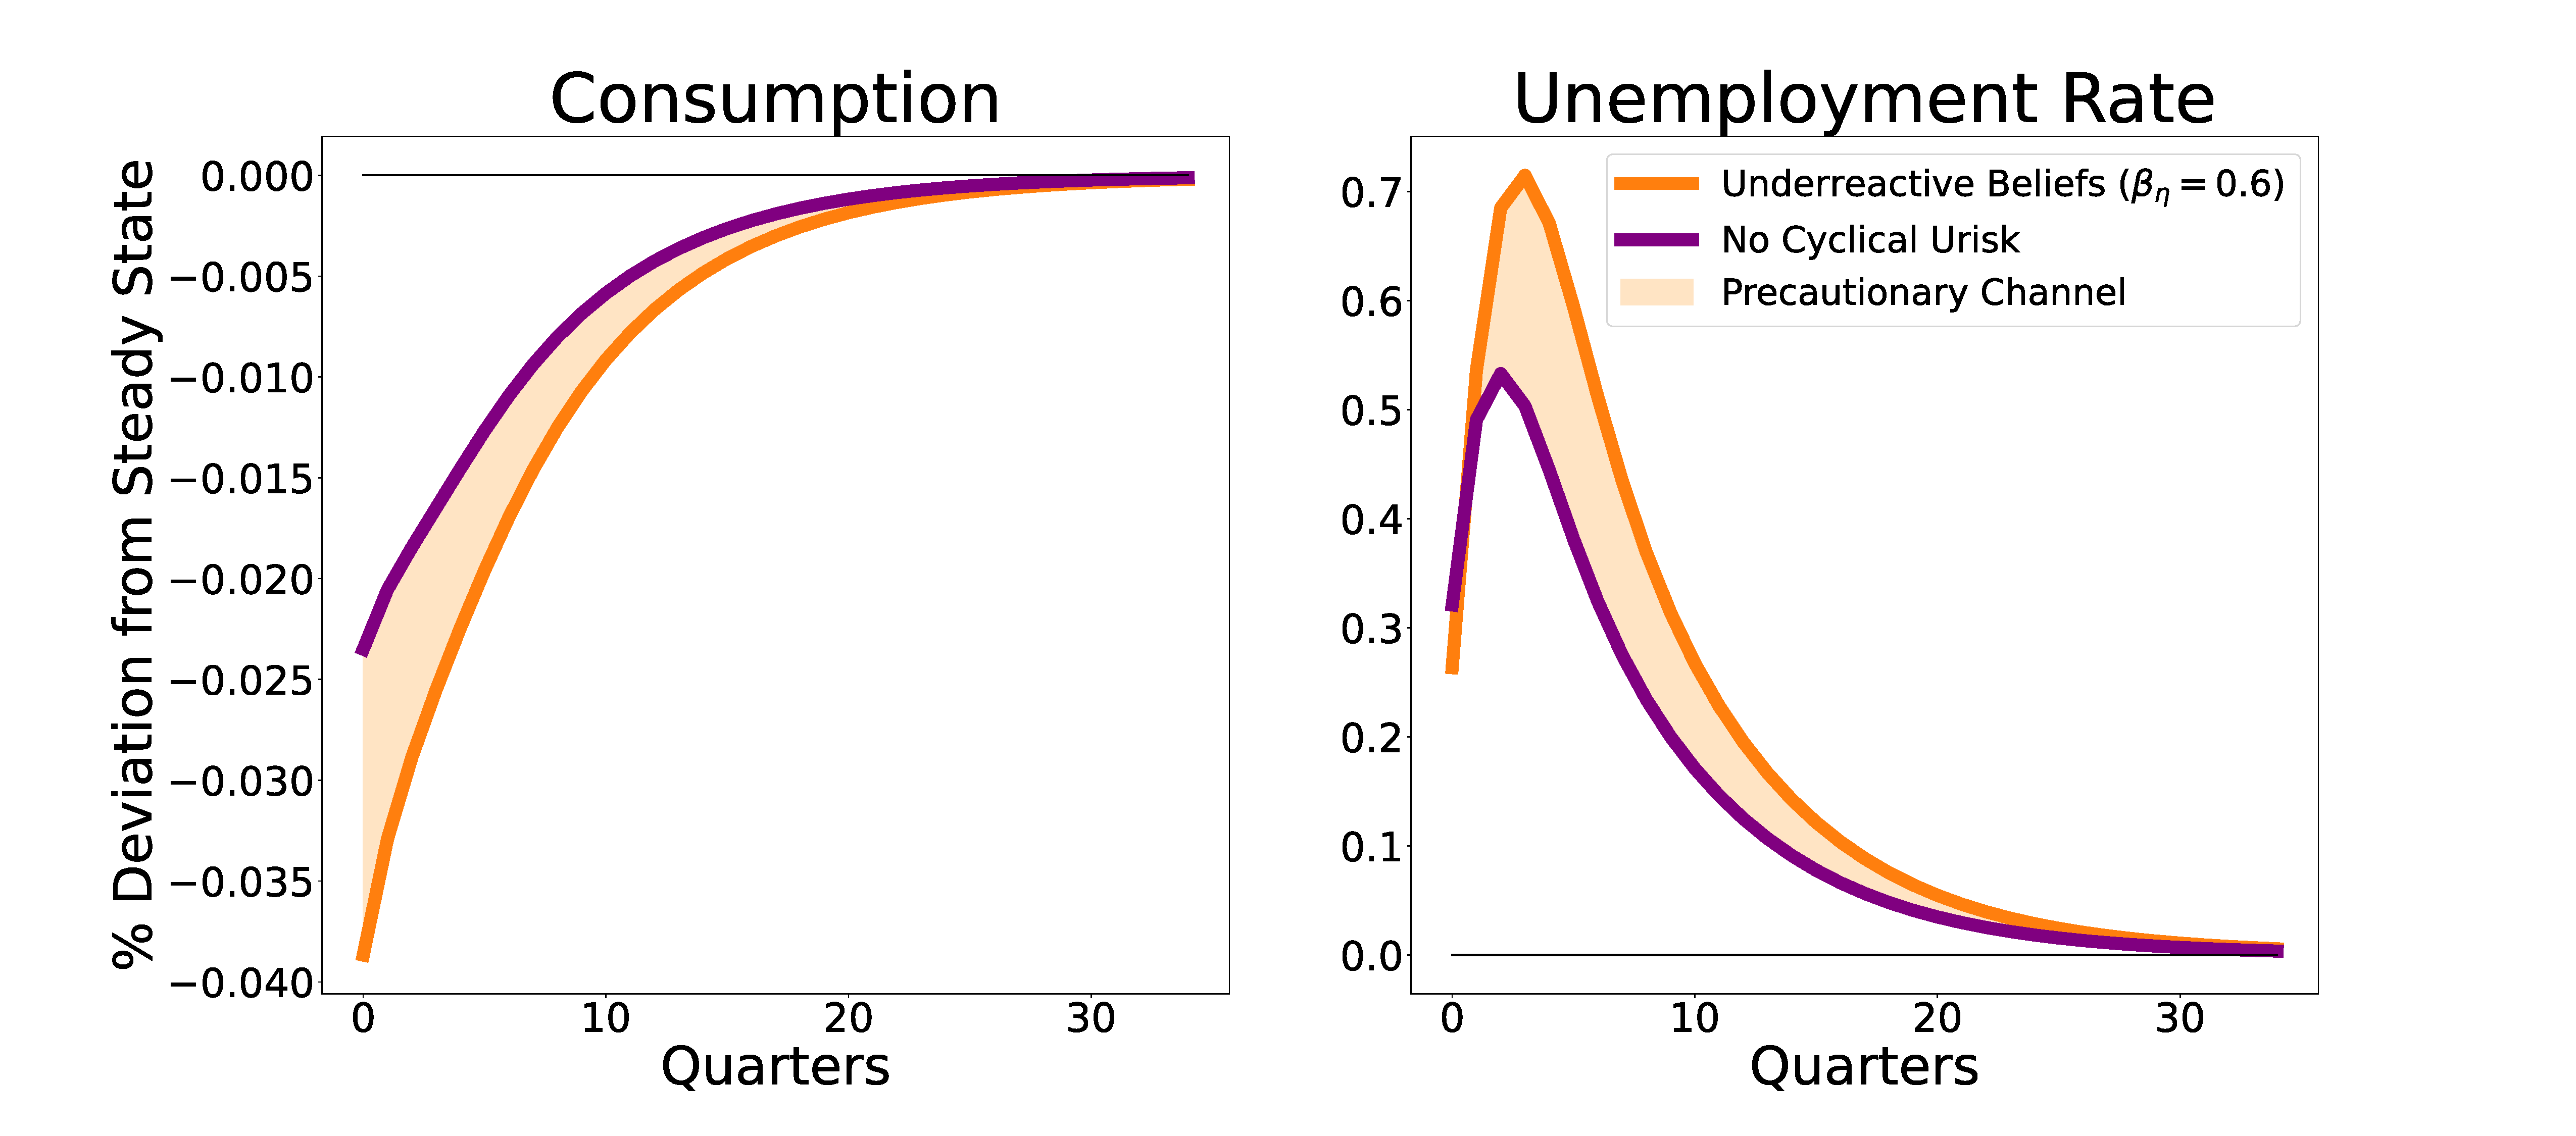
\includegraphics[scale=.15]{\FigDir/Precautionary_Channel}
%     \label{fig:Precautionary_Channel}
%\end{figure}

Figure \ref{fig:IPR_ev_Urisk} plots the impulse responses to a monetary policy contraction of the baseline model, and a model with no cyclical unemployment risk. In particular, I compare a model with underreactive beliefs and a model where households do not change their precautionary savings in response to changes in unemployment risk. The difference in volatility between the impulse responses of these models is the precautionary channel. While the volatility of the impulse responses of the economy with underreactive beliefs are attenuated compared to the model with rational beliefs, the model still demonstrates sizeable amplification through the precautionary channel. In particular, the share of fluctuations in aggregate consumption and the unemployment rate due to the precautionary channel. In particular, the precautionary channel is large and accounts for 46\% of the variance in the unemployment rate response and 60.5\% of the variance in the aggregate consumption response. \\

\hypertarget{The Role of Shock Persistence}{}
\section{The Role of Shock Persistence}

In this section I clarify the role of the persistence of a monetary policy shock in explaining the size of the precautionary channel. \\


\begin{figure}
    \centering
     \caption{ Precautionary Multiplier and Channel Share Across Shock Persistence }
    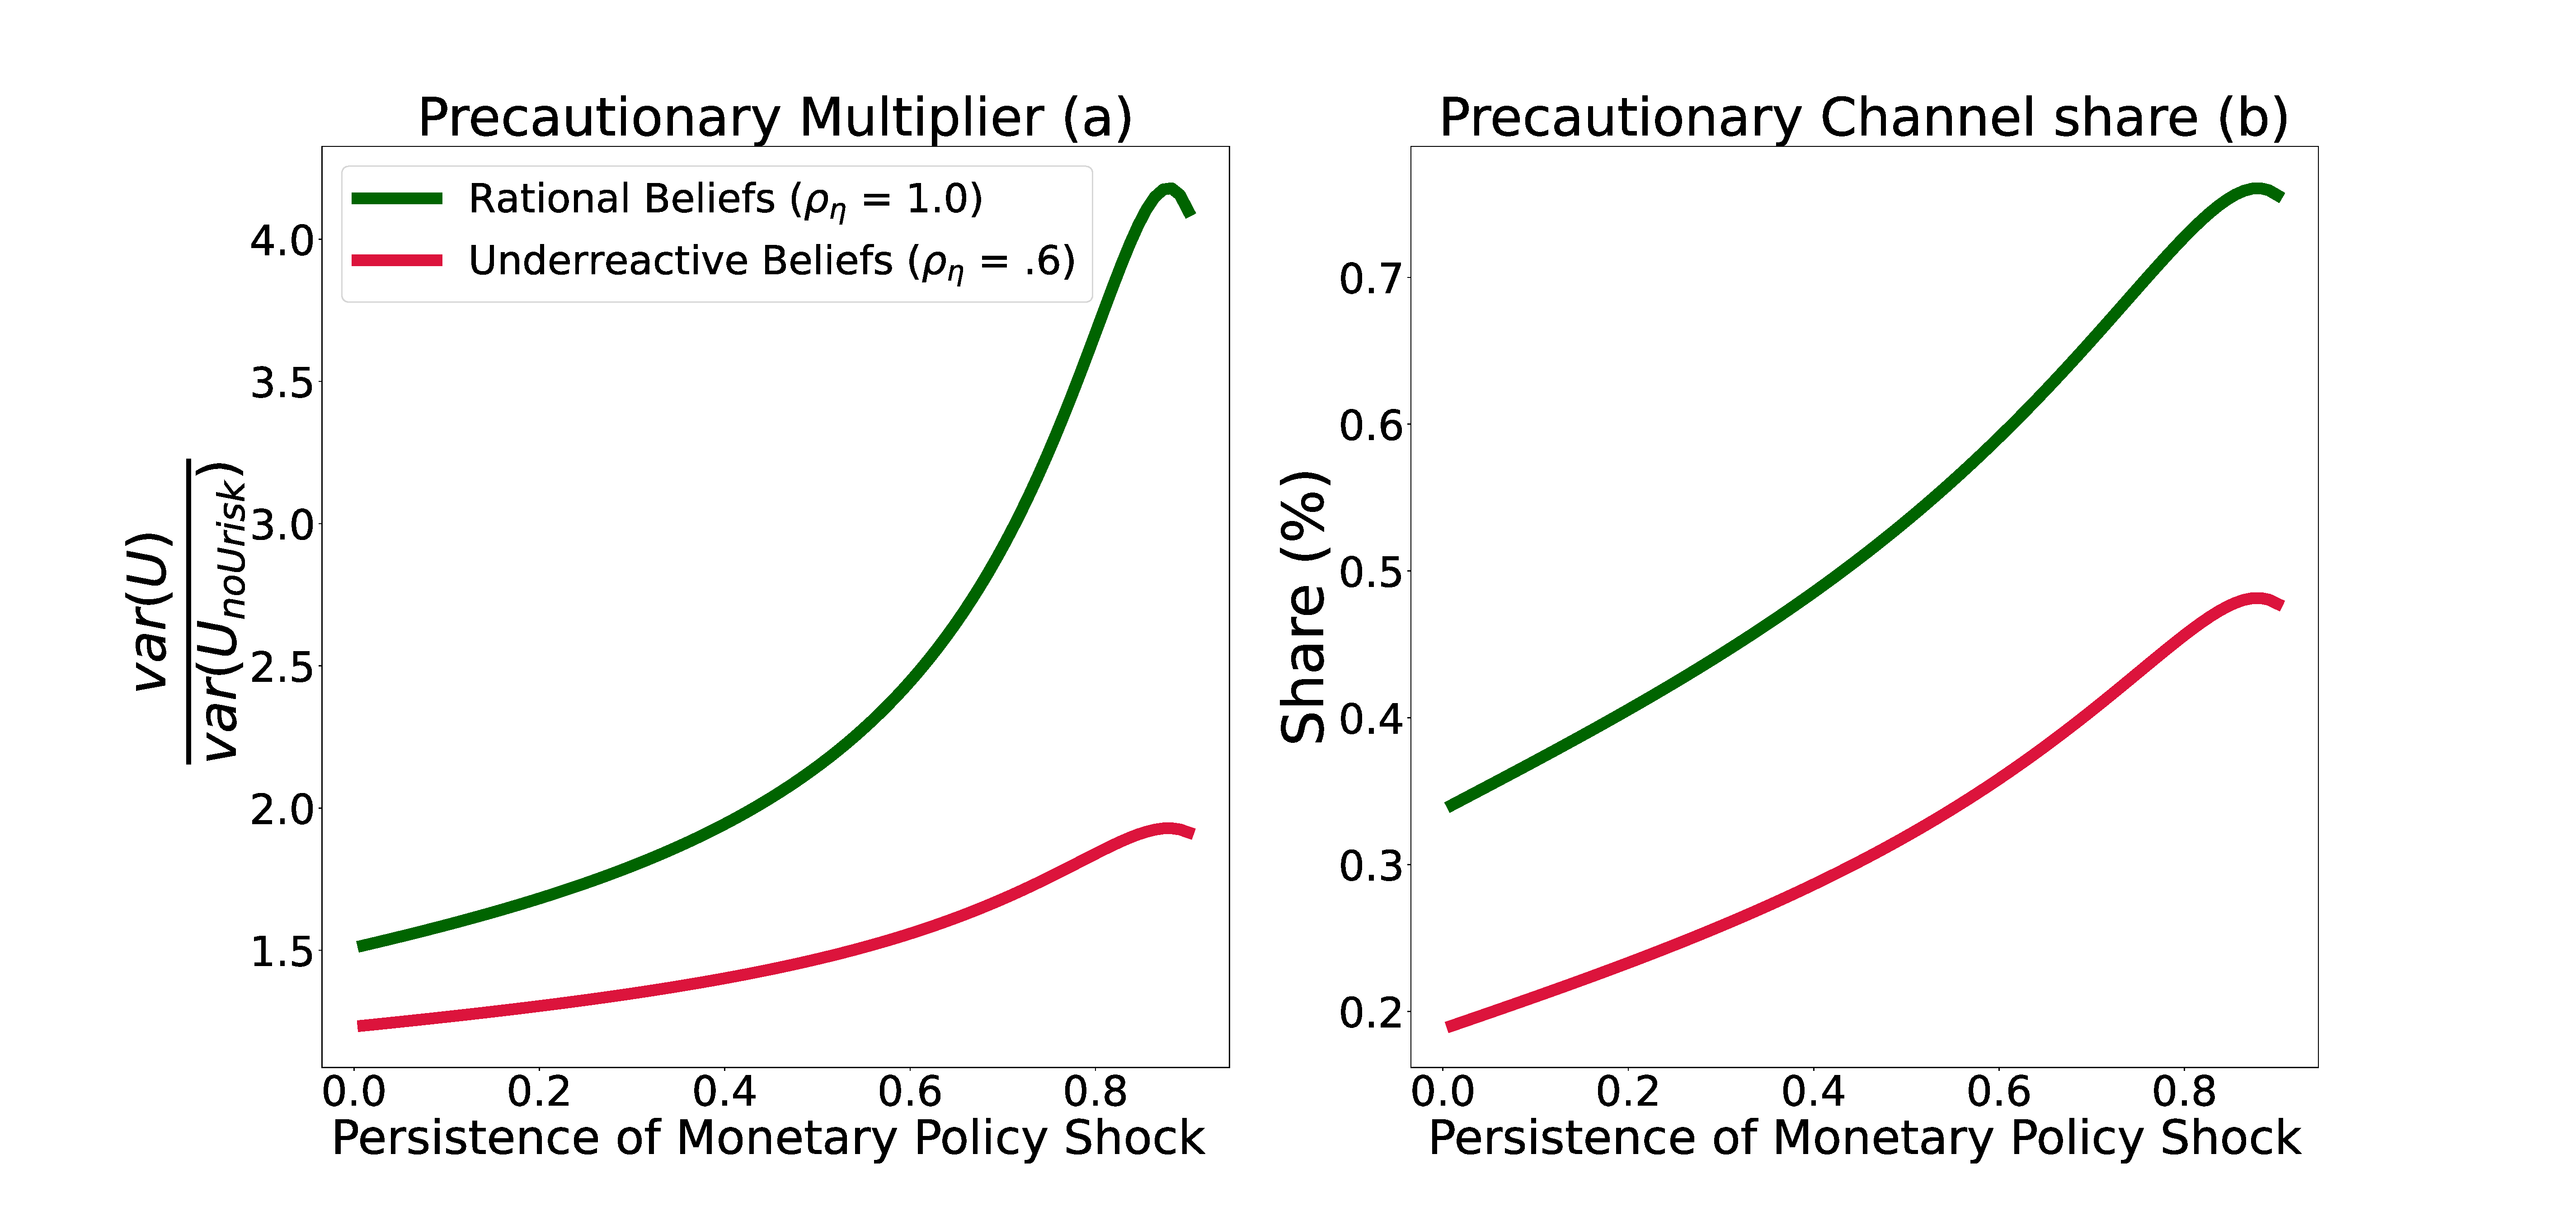
\includegraphics[scale=.15]{\FigDir/Multipliers}
     \label{fig:Multipliers}
\end{figure}

Figure \ref{fig:Multipliers} illustrates the role of shock persistence on the amplification of the precautionary channel. Graph (a) plots the the ratio of the variance of the unemployment rate response in the baseline model to the variance of the unemployment rate response in the model with no cyclical unemployment risk across monetary policy shock persistences. I define this ratio to be the precautionary multiplier. Graph (b) plots the share of variance in the unemployment rate response due to the precautionary channel across monetary policy shock persistences. The plots demonstrate that the increased volatility due to the precautionary channel increases exponentially with the persistence of the shock while a larger share of the increased volatility is attributed to the precautionary channel. Overall, the amplification of the volatility of the business cycle through precautionary saving rises with the persistence of the monetary policy shock.\\





\begin{figure}[H]
    \centering
    \caption{Partial Equilibrium Consumption Response to AR(1) Shocks }
    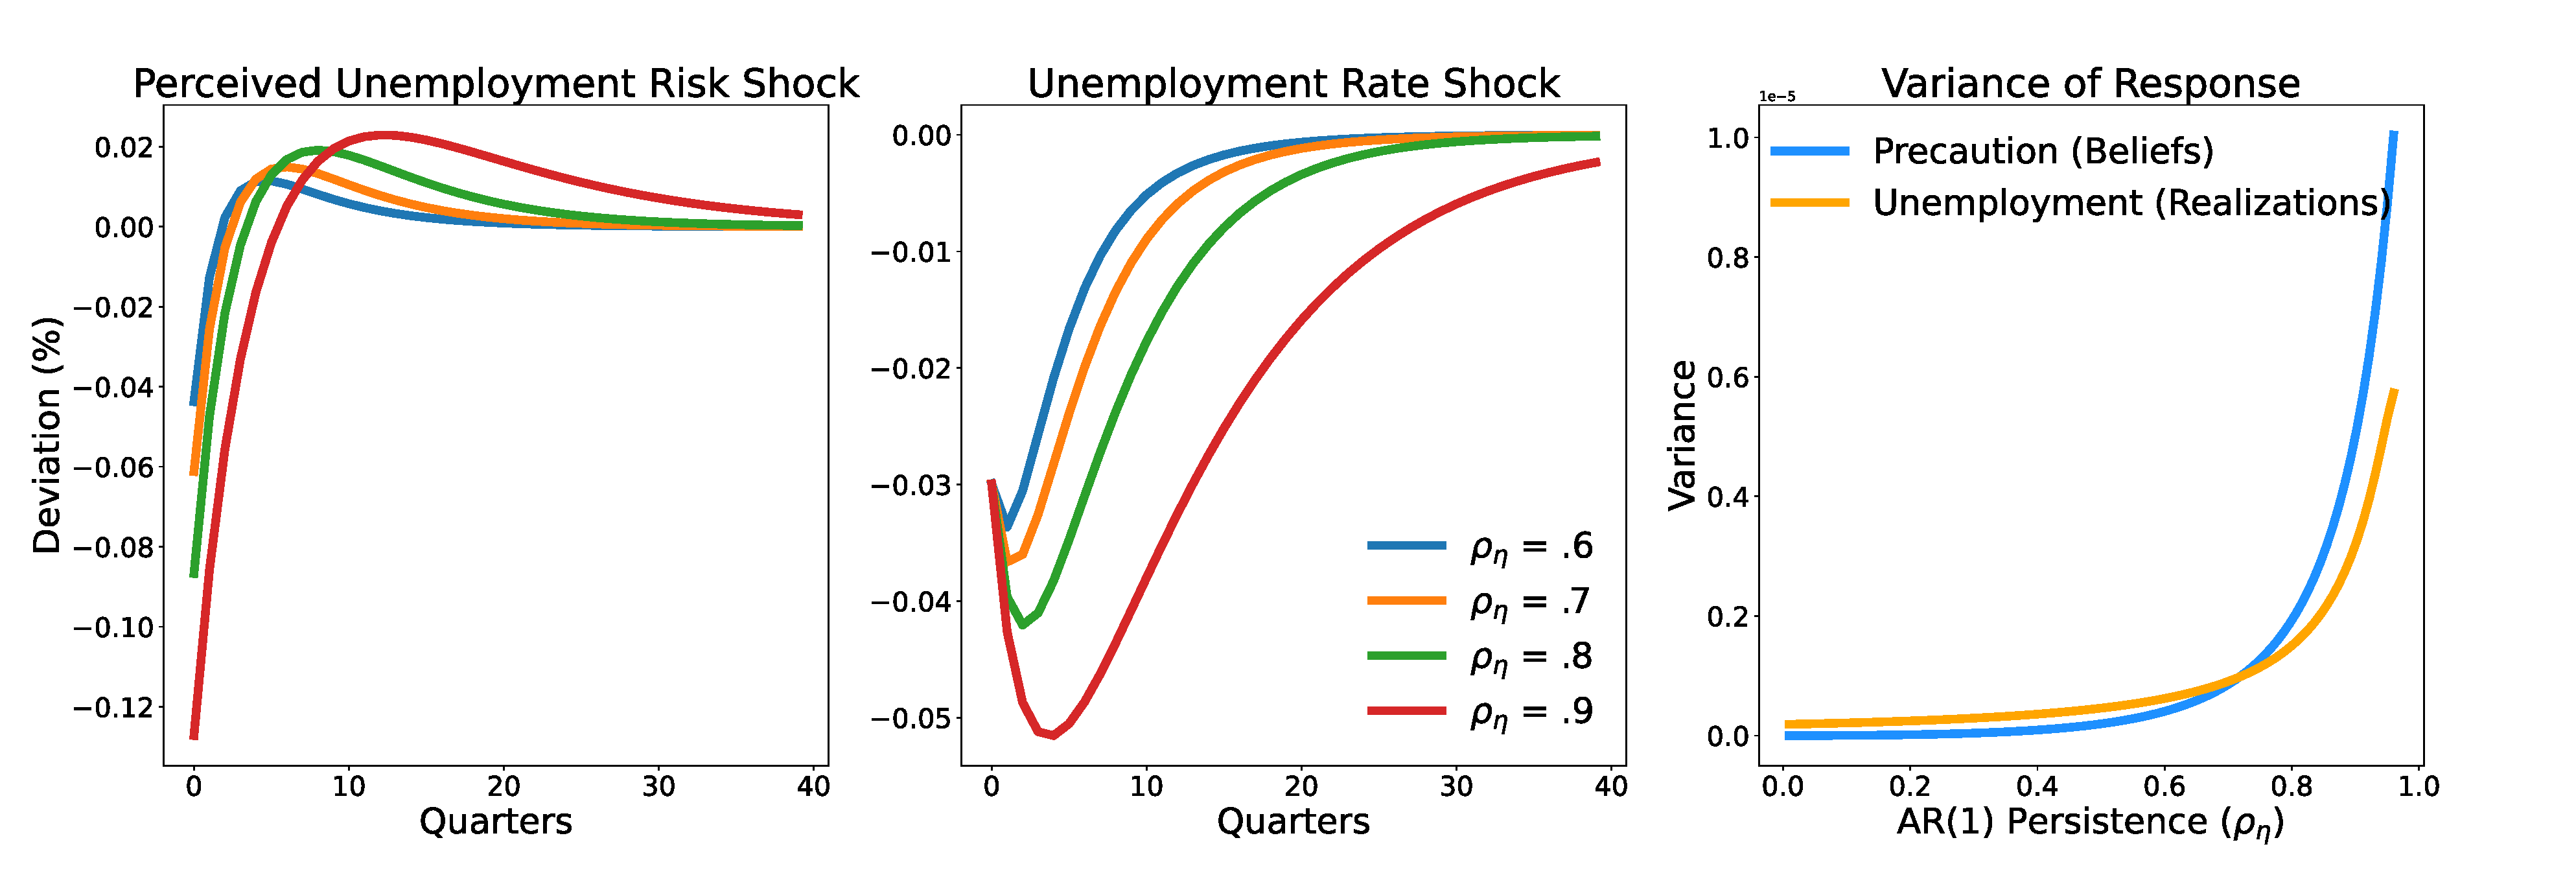
\includegraphics[width=\linewidth, height=\plotheight\textheight]{\FigDir/Duration_Precaution_crop}
    \floatfoot{Note: The first two panels plot the partial equilibrium impulse responses of consumption to AR(1) shocks at differing shock persistences $\rho_{\eta}$. The first panel plots the impulse response to a shock to job finding beliefs while the second panel plots the response to a shock to the realized job finding probability assuming households never perceive the job finding probability to change. The last panel plots the variances of the responses of consumption across different shock persistences. }
    
    %A shock to the job finding probability affects both unemployment risk and the unemployment rate. The first panel considers the effect of job finding probabilities on consumption through changes in the unemployment risk while the second panel considers the effect of job finding probabilities on consumption through changes in the unemployment rate. The last panel plots the variances of the responses of consumption across different shock persistences.  }
     \label{fig:C_Responses}
\end{figure}



The exponential rise of the precautionary multiplier stems from both the sensitivity of the precautionary motive to the persistence of heightened unemployment risk and the interaction of this sensitivity with the persistence in the IMPCs. The first two panels in figure \ref{fig:C_Responses} illustrate the partial equilibrium impulse responses of consumption to AR(1) shocks of varying persistences on job finding beliefs (perceived unemployment risk)\footnote{AR shocks to job finding beliefs are effectively shocks to perceived unemployment risk and therefore the consumption response captures the precautionary response to heightened unemployment risk.} and job finding realizations (unemployment rate)\footnote{AR shocks to job finding realizations are shocks to the unemployment rate as the job finding probability dictates the mass of individuals who will transition into unemployment.}.  I study the response of aggregate consumption as it amplifies the business cycle through nominal rigidities (Demand determined output). The shocks to perceived unemployment risk (first panel) illustrate that the precautionary motive is sensitive to the duration of heightened unemployment risk with the impact of the shock increasing exponentially with the persistence of the shock. The consumption response to shocks to the unemployment rate (second panel) are also sensitive to the persistence of the shock however the initial impact of all shock persistences are the same because the size of shocks are all the same. Under shocks to the unemployment rate, the persistence of the consumption responses differ with persistence due to the slow decay of the IMPCs. The longer the duration of heightened unemployment causes persistence in losses to aggregate income which leads the consumption response to persist. To quantify and compare the exponential rise of both shocks across persistence, the third panel plots the variance of consumption to both perceived unemployment risk shocks and unemployment rate shocks. The panel illustrates the exponential rise in the variance of consumption for both shocks with the perceived unemployment risk shocks (Blue Line) increasing at a greater rate than the unemployment rate shock. \\


\begin{figure}[H]
    \centering
      \caption{Variance of Consumption Responses in General Equilibrium}
    \includegraphics[scale=.8]{\FigDir/Variance_Bf}
      \floatfoot{Note: This figure plots the variances of the general equilibrium consumption response to the endogenous changes in perceived unemployment risk and the unemployment rate. These plots are the general equilibrium counterparts of the third panel in figure \ref{fig:C_Responses}}
     \label{fig:Variance_GE}
\end{figure}


Figure \ref{fig:Variance_GE} illustrates the variances of consumption to both heightened unemployment risk and increased unemployment in general equilibrium. In general equiilbrium, the endogenous path of the job finding probability does not follow an AR(1) and therefore the graph is plotted across different monetary policy shock persistences to capture the resulting general equilibrium paths of unemployment risk and unemployment. The rise in the variances are amplified due to their interaction in general equilibrium. Comparing the rise in the variance due to the unemployment effect between the baseline model (Orange) and model with no cyclical unemployment risk (Maroon), the dramatic rise in the variance attributed to the unemployment effect stems from its interaction with the precautionary effect. The addition of precautionary saving magnifies the initial drop in aggregate consumption as households immediately build a larger precautionary buffer stock upon learning of the shock.  This decline in consumption transmits through output and raises the unemployment rate which proliferates the fall in consumption because of the persistence in the IMPCs. With the precautionary motive rising sharply with the persistence of heightened unemployment risk, the intensity of the proliferation in consumption from the interaction between persistent IMPCs and precautionary saving rises further with the persistence of the monetary policy shock.


%\footnote{In the calibration with $\beta_\eta = 1.0$, in the right panel, the precautionary component rises much more sharply than the unemployment component.} 
%%Figure \ref{fig:Persistence} plots the decomposition of the variance of consumption to varying shock persistences in both partial and general equilibrium. Consumption is decomposed into a precautionary and unemployment (income loss)\footnote{ A decline in the job finding probability raises unemployment rate reducing consumption as households lose their wage and claim unemployment benefits} component \footnote{I exclude the effect of the interest rate and taxes on aggregate consumption. Including these components do not add to the point made and complicated the figures}. I study the variance of the response to aggregate consumption because demand determined output is crucial for the amplification of the model. The partial equilibrium graph plots the variance of the components of aggregate consumption to AR(1) shocks of varying persistences to the job finding probability. In partial equilibrium, the precautionary effect is more sensitive to a shock's persistence than the unemployment effect. This is because households precautionary motive intensifies with the duration of heightened unemployment risk. Although, the unemployment component demonstrates weaker sensitivity than the precautionary component, aggregate income loss from rising unemployment still generates an exponential rise in the unemployment component with a shock's persistence due to the slow decay of the IMPCs. In particular, newly unemployed households will significantly reduce their consumption on the impact of their unemployment spell and continue to reduce their consumption in the following periods at a decaying rate. With the persistence in the unemployment rate response rising with the shock persistence, this causes the fall in consumption to proliferate. 













%%
%\begin{figure}{}
%    \centering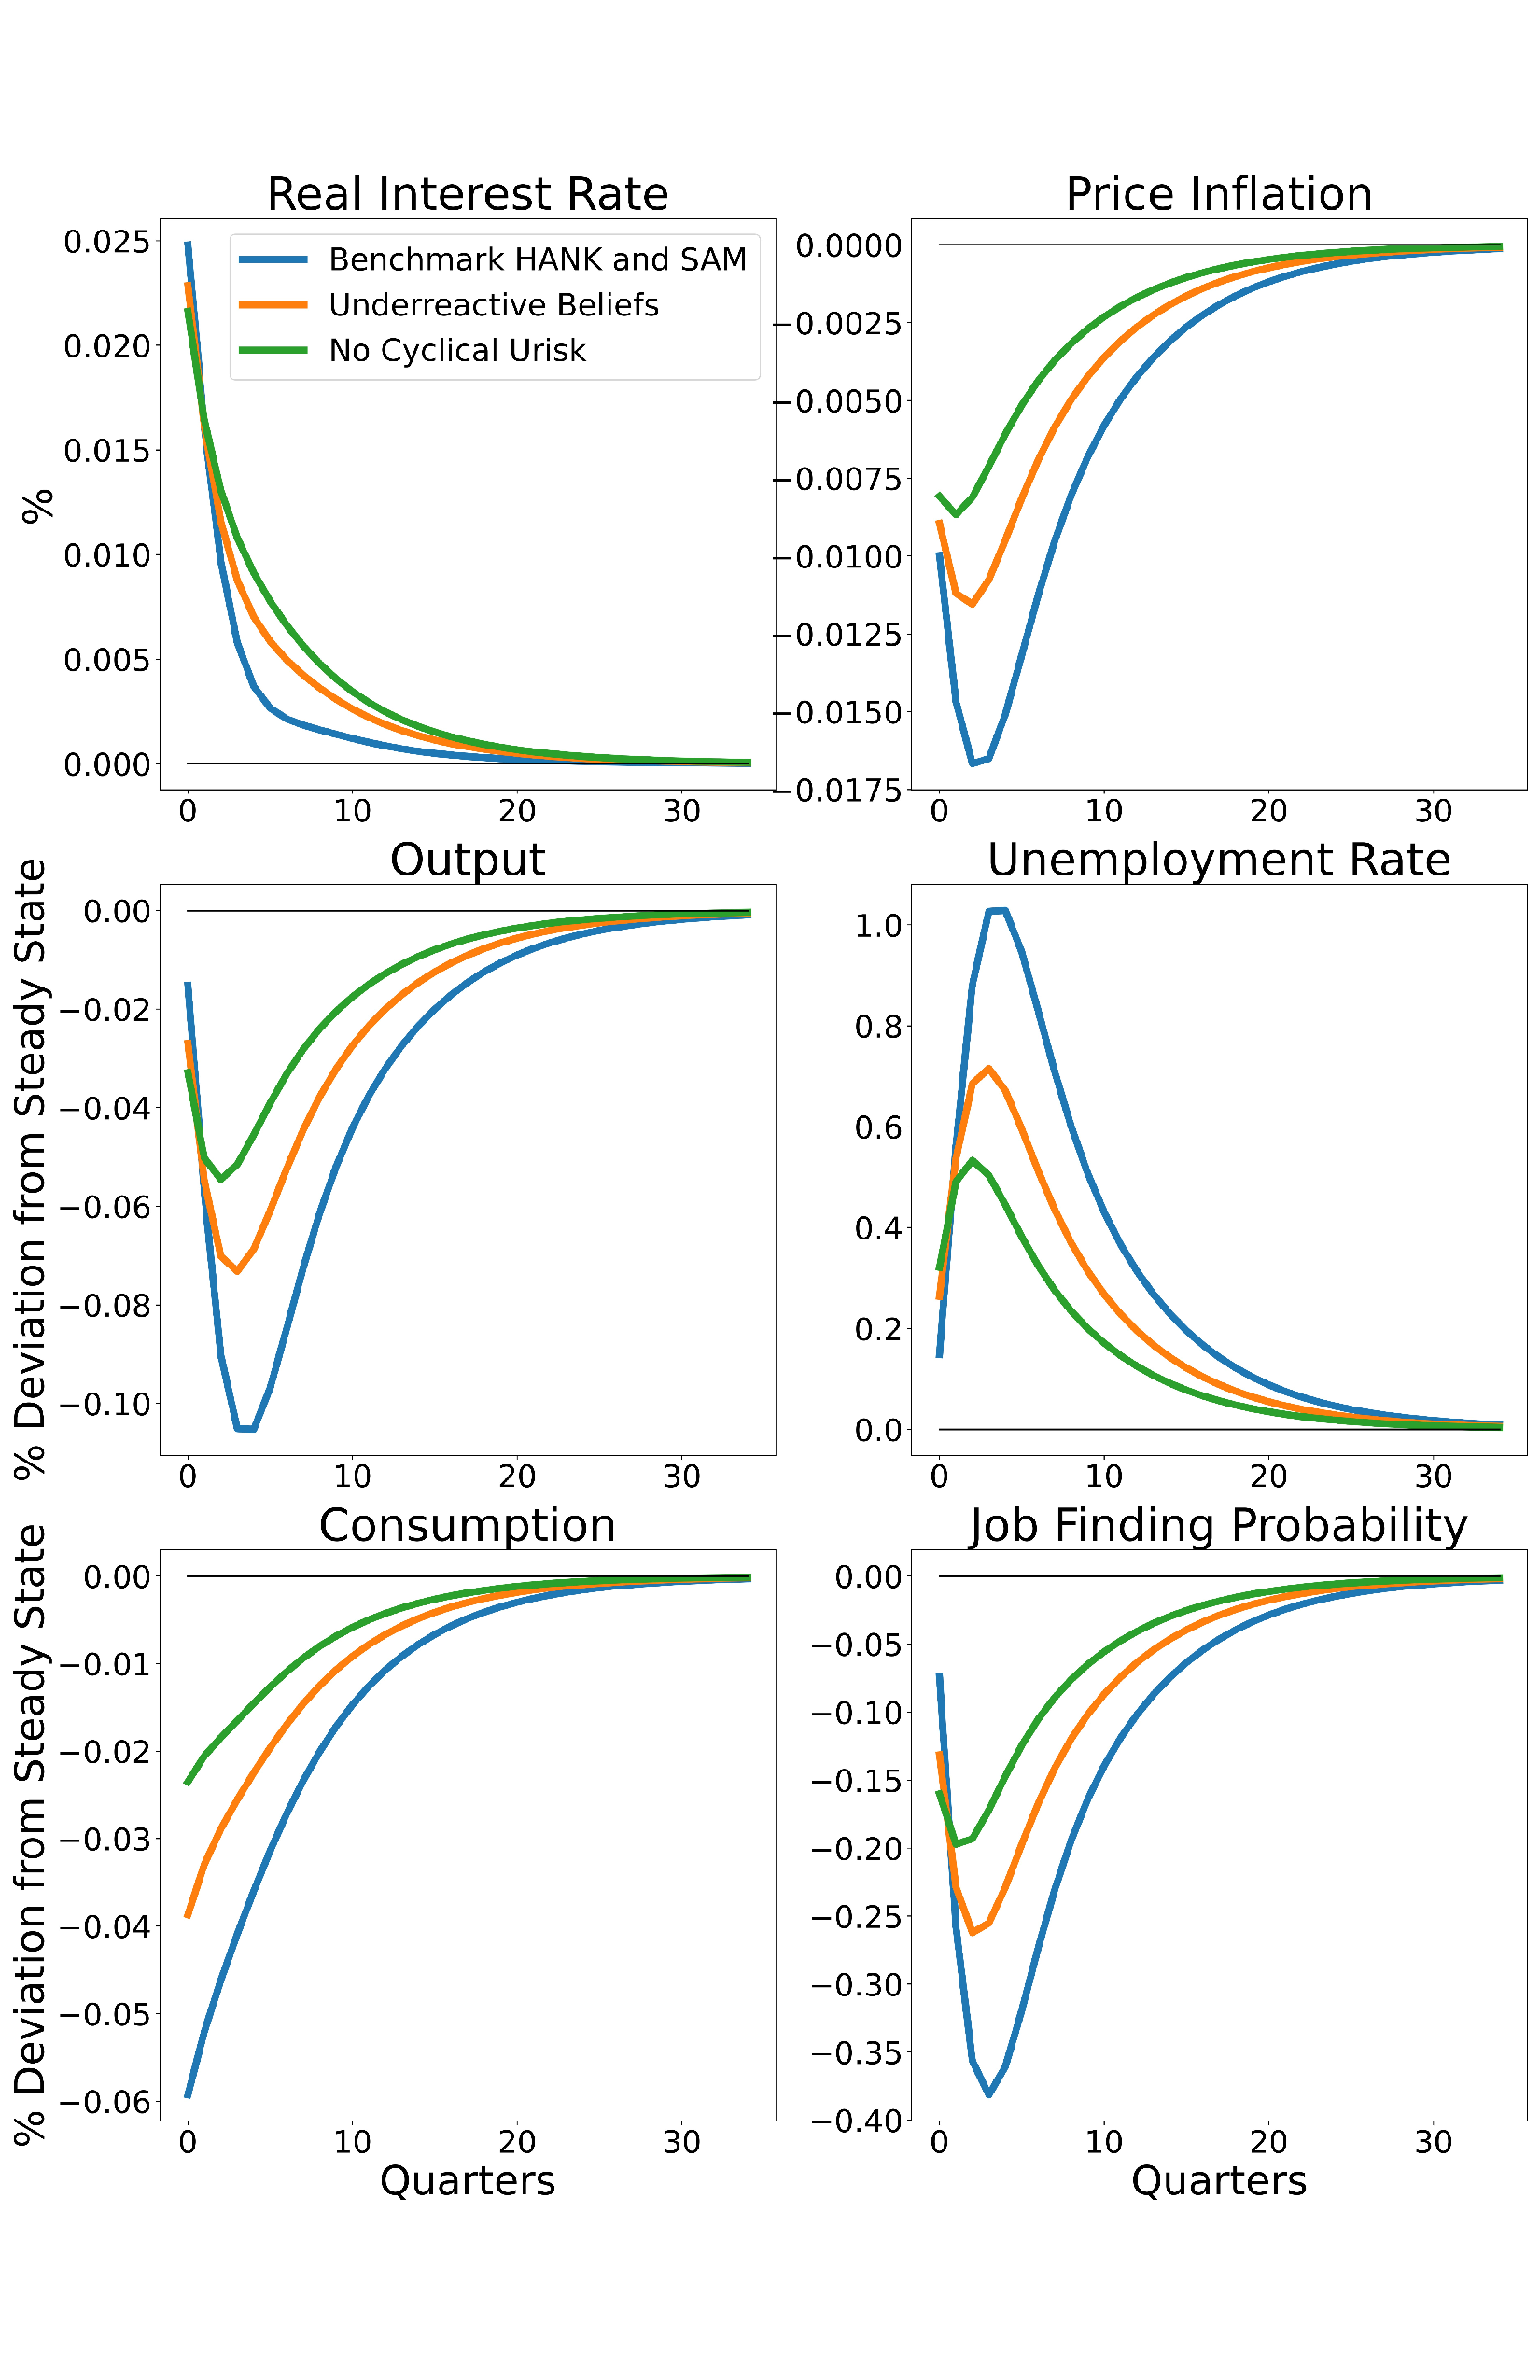
\includegraphics[scale=.5]{\FigDir/Impulses_ev}
%    \caption{Impulse Responses to Monetary Contraction Shock }
%     \label{fig:IPR_ev}
%\end{figure}
%%


%\begin{figure}{}
 %   \centering\includegraphics[scale=.5]{\FigDir/C_breakdown}
 %%   \caption{Consumption Breakdown }
%\end{figure}
%\hypertarget{Shock to Job Finding Beliefs }{}
%\section{Shock to Job Finding Beliefs }

%\begin{figure}{}
%    \centering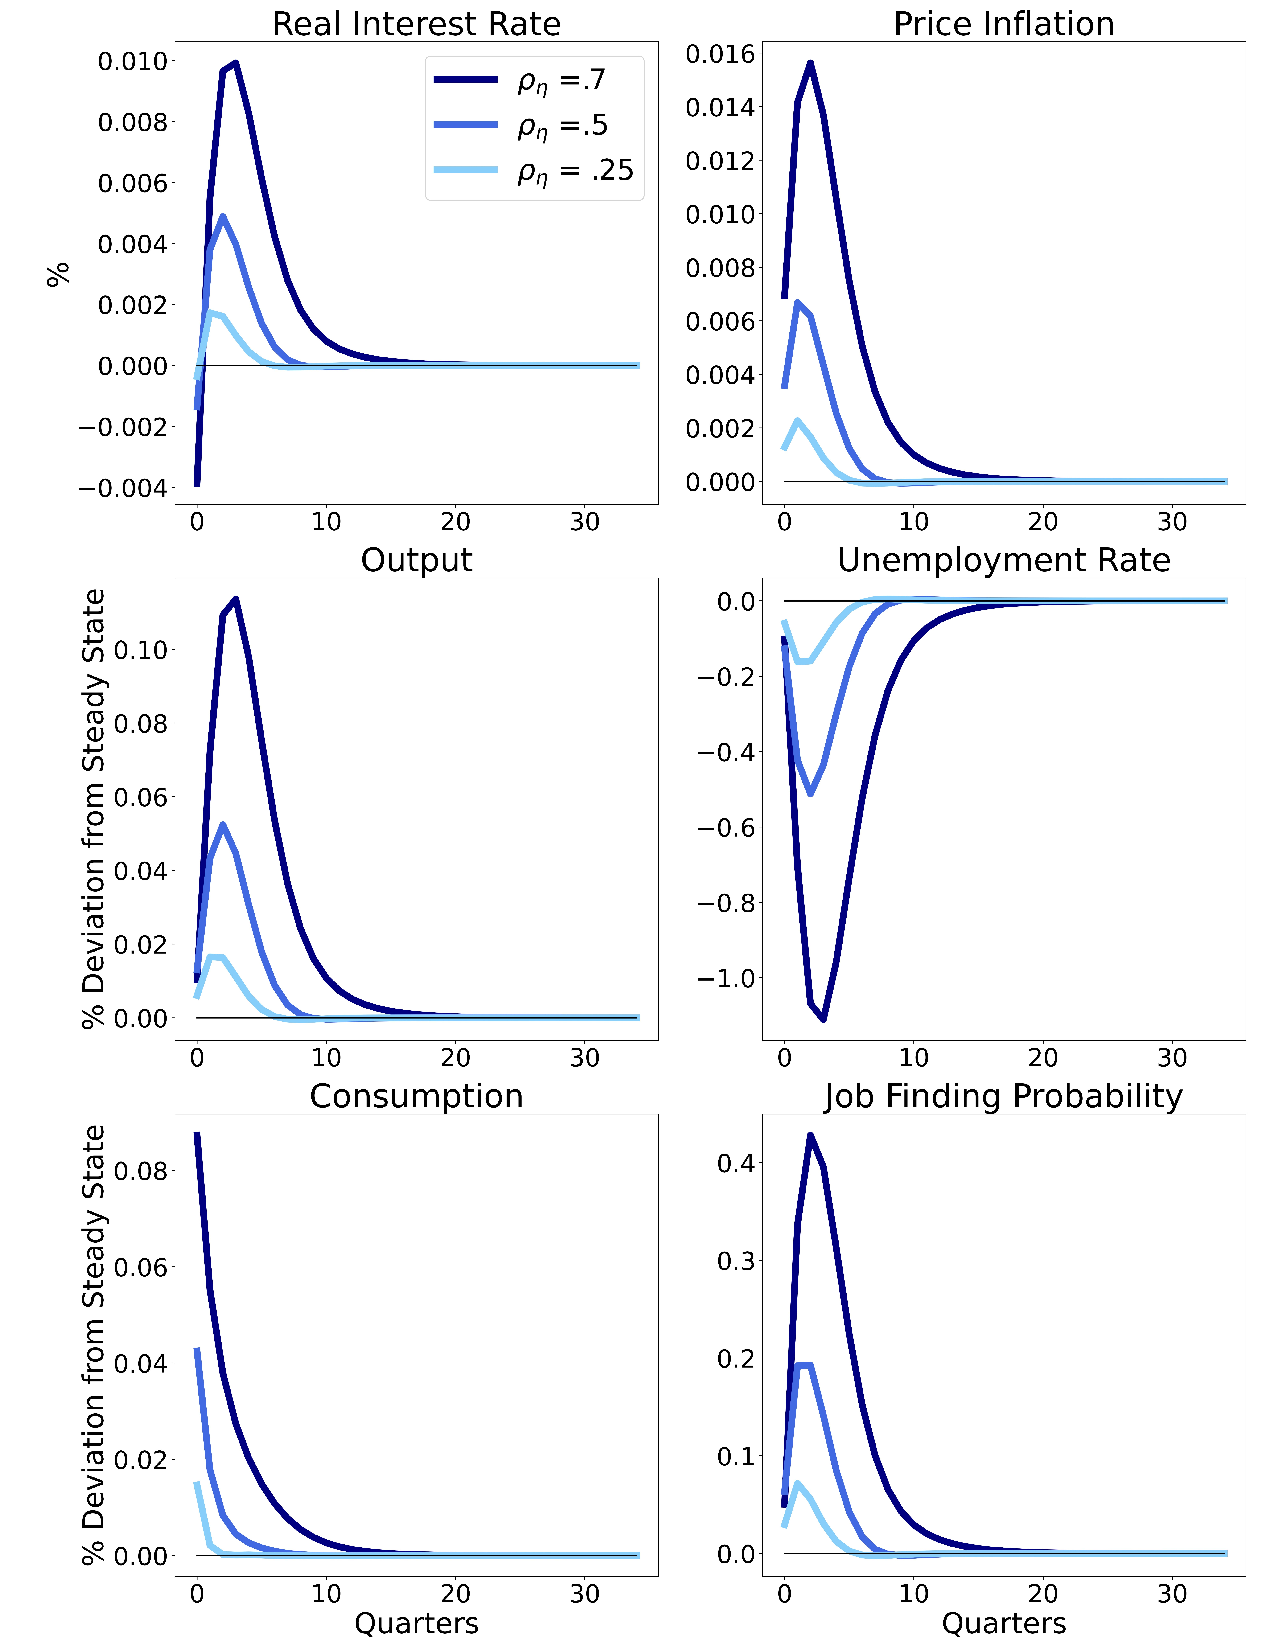
\includegraphics[scale=.8]{\FigDir/IPR_e_bf}
   % \caption{Impulses Responses to Job Finding Beliefs Shock }
%\end{figure}





\hypertarget{Looking Forward }{}
\section{Looking Forward }

Looking forward, I plan to compute the consumption and savings jacobians across distribution of wealth to determine the effect of uncertainty across the cross section of wealth. In particular, I may compute the consumption jacobian to a unemployment risk shock for the bottom third of the wealth distribution and compare it to the jacobian of the whole economy to determine whether a particular part of the distribution is driving the results. I am also thinking of expanding the modeling of unemployment insurance to be more realistic. In particular, at the moment, unemployed households receive unemployment benefits no matter the duration of their unemployment spell. This is clearly not realistic and therefore I plan to have unemployment benefits only lasting two periods into the unemployment spell. With a more realistic model of unemployment insurance, I may study shocks to unemployment benefit duration since the precautionary channel is sensitive to the persistence of unemployment risk. Furthermore, I may solve an analytical HANK and SAM commonly used in the literature to demonstrate the importance of full fledge heterogeneity on the results of the model. Finally, this dissertation proposal may split into two separate avenues. This paper concerns the role of precautionary saving over the business cycle and the determinants of this this channel in a full fledged HANK model. The addition of beliefs lends a more realistic calibration of beliefs however I believe the inclusion of job separation expectations could lead to an interesting result in its own right, away from the analysis of the sensitivity the precautionary channel. Thus, I may pursue a separate paper that includes both job finding expectation and job separations data and analyze how the model discpline by expectations data differs than its rational counterpart. In such a framework, as a first basis, I would estimate a shock series from the job separation expectations and simulate the model with those shocks to determine any differences.





%%\begin{figure}{}
   % \centering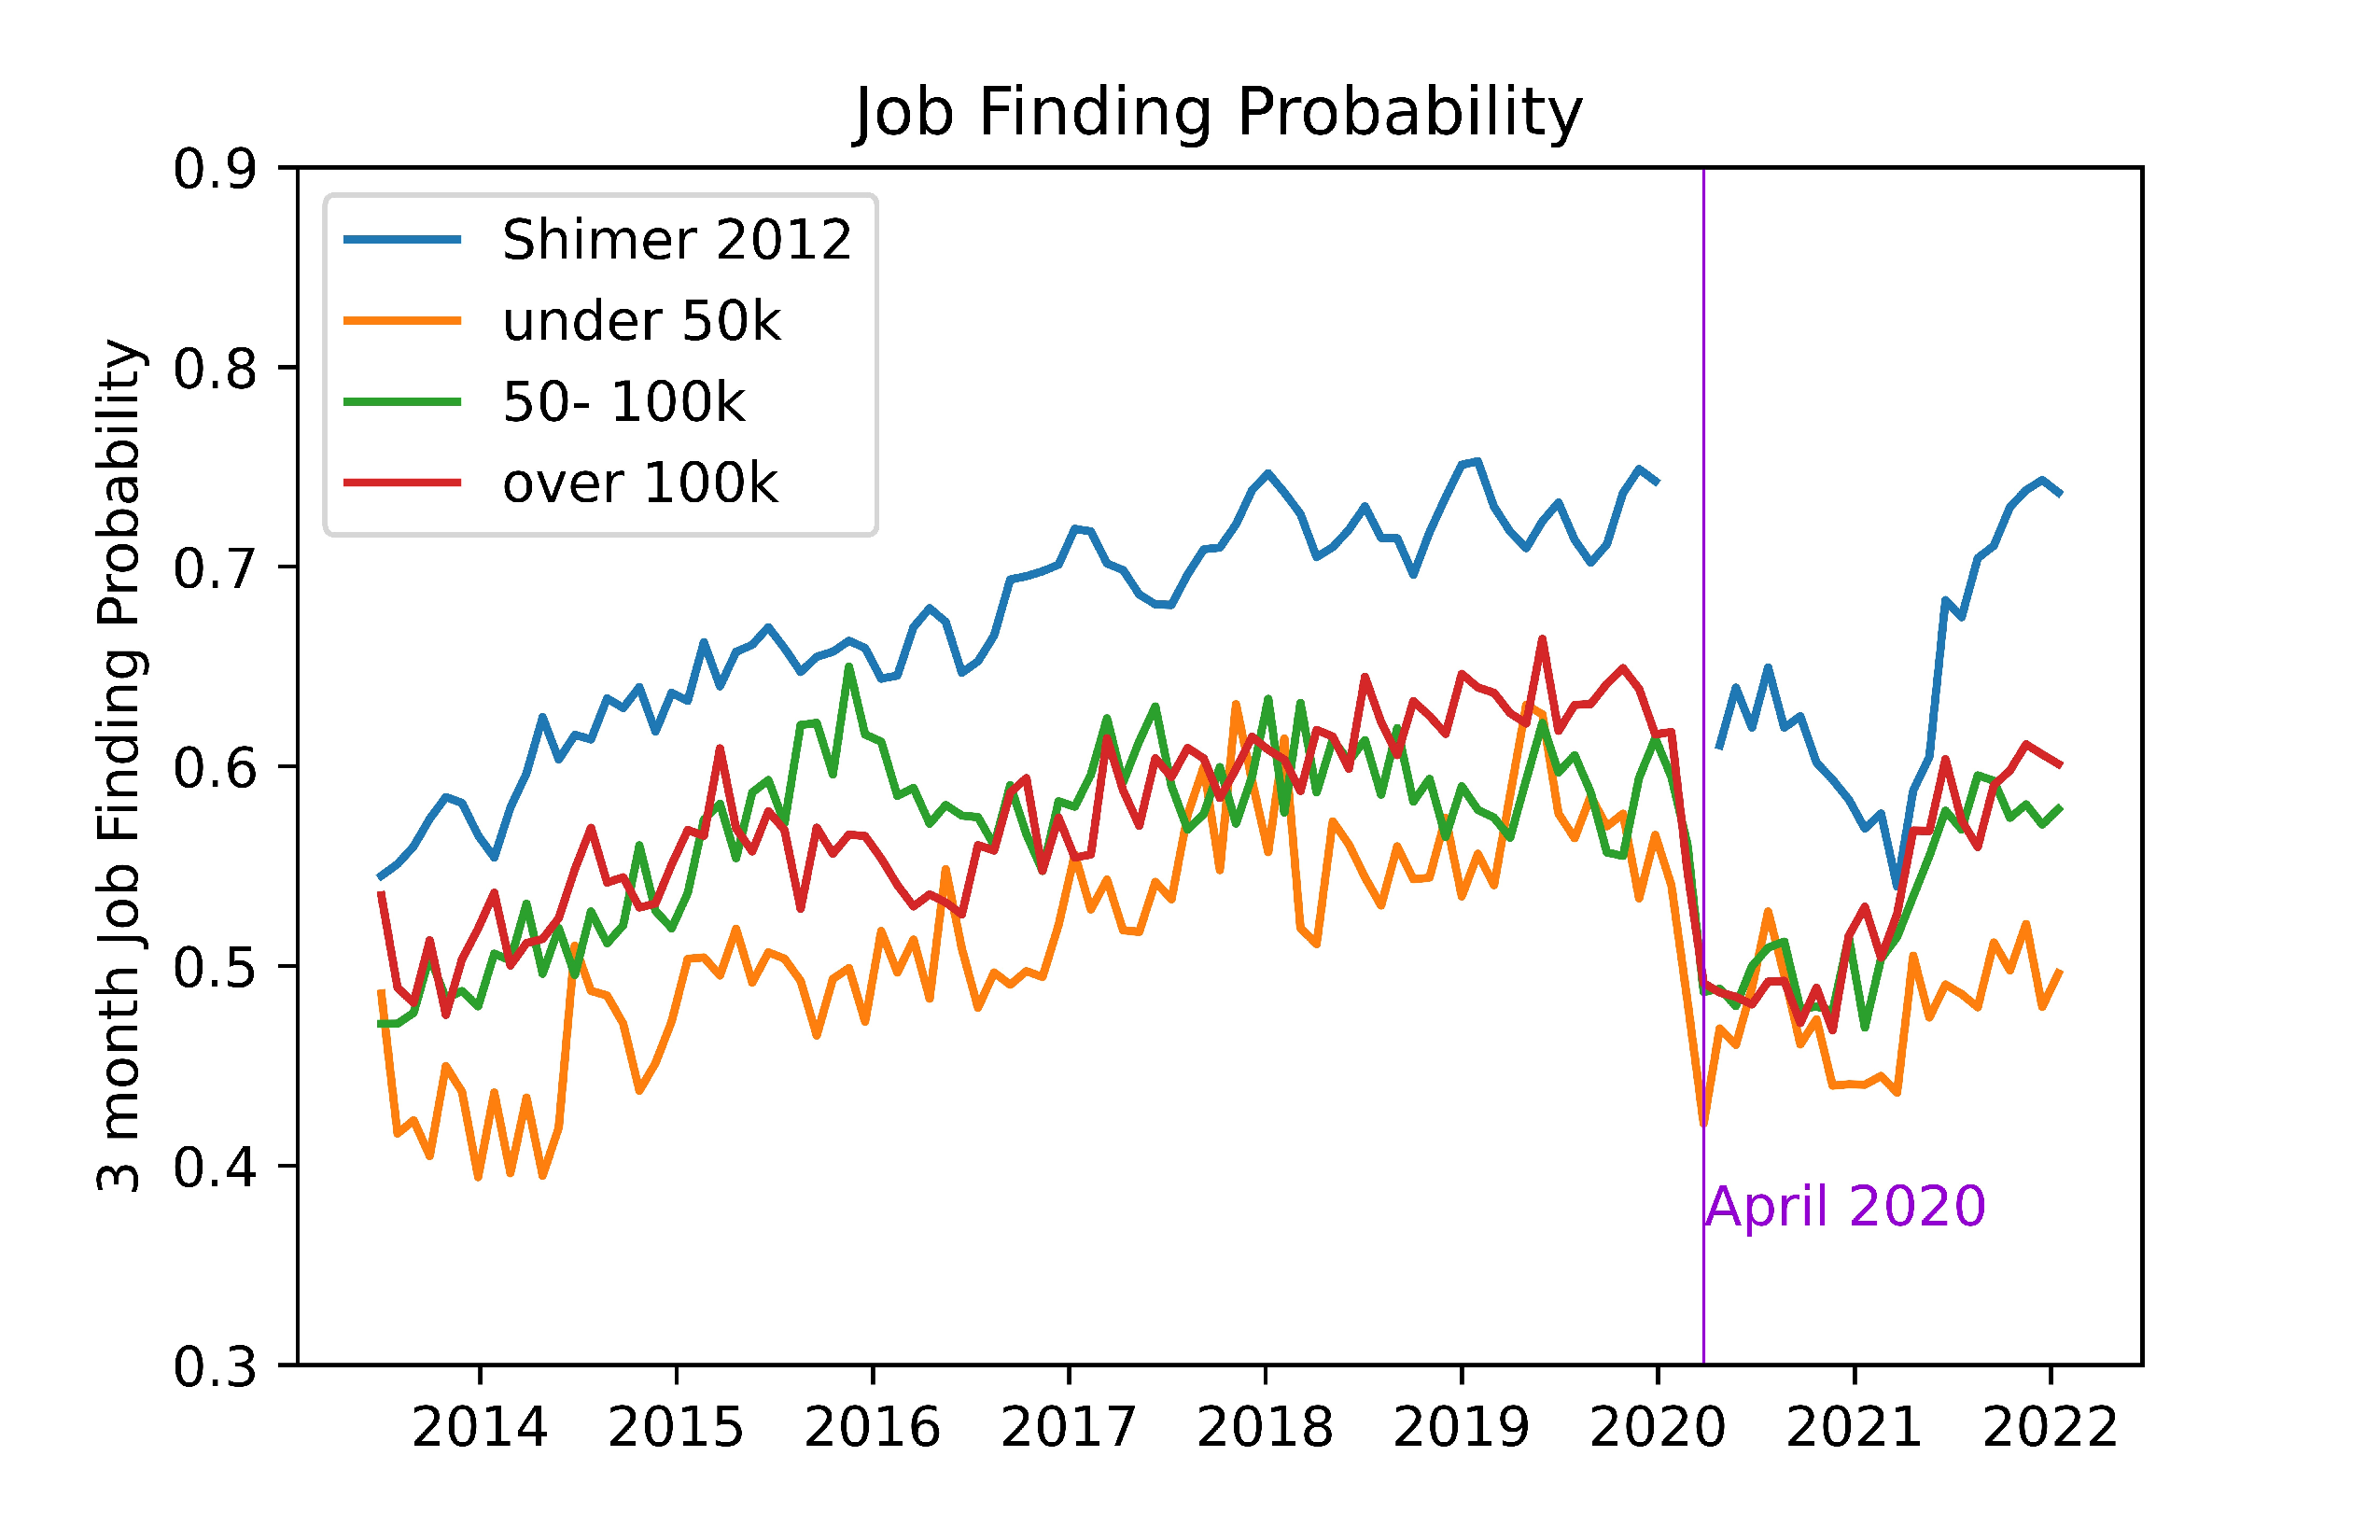
\includegraphics[scale=.26]{\FigDir/HetJF}
    %\caption{Comparison of expectations of 3 month job finding across Income Groups. }
%\end{figure} 
%%It may also be interesting to explore the consequences of heterogeneous beliefs across income (see figure 4 for a plot of expectations of job finding across income). Given households with lower levels of liquidity are more sensitive to fluctuations in unemployment risk (\cite{heathcote2018wealth}), it may be interesting to investigate the interaction between heterogeneous beliefs in job transition probabilities and distribution of wealth. If low income households face sharper changes in unemployment risks than middle and high income households, then the change in aggregate consumption would be amplified relative to a baseline HANK model where all households face the same unemployment prospects as the low income households would have an even stronger precautionary savings motive.









%\providecommand{\figName}{GIPRM1}
%\providecommand{\figFile}{GIPRM1}
%\hypertarget{\figFile}{}
%\hypertarget{\figName}{}
%\begin{figure}[tbp]
%\centerline{\includegraphics[scale=.35]{\FigDir/\figFile}}
%\caption{Monetary Policy Shock}
%\label{fig:\figFile}
%\end{figure}


%%
%\renewcommand{\figFile}{GIPRM2}
%\hypertarget{\figFile}{}  
%\begin{figure}[tbp]
%\centerline{\includegraphics[scale=.35]{\FigDir/\figFile}}
%\caption{Monetary Policy Shock}
%\label{fig:\figFile}
%\end{figure}
%%


\clearpage\vfill\eject







%%Now let $v(m_{it}, c_{it}) = \frac{c_{i t}^{1-\rho}}{1 -\rho} - \varphi \frac{n_{it}^{1+v}}{1+v} + \beta_{i}\not D \mathrm{E}_{t}[\psi_{it+1}^{1-\rho} V(m_{it+1})] $ and let $c_{it}(m_{it})$ denote the solution to the original dynamic problem.  \\ 

%%Note $ \frac{ \partial v(m_{it},c_{it}(m_{it}))}{\partial m} =  \beta_{i}\not D \mathrm{E}_{t}[\psi_{it+1}^{1-\rho} V'(m_{it+1})] $ \\

%%Then $$ V(m_{it}) = v(m_{it}, c_{it}(m_{it})$$ 

%%$$ V'(m_{it}) = \frac{ \partial v(m_{it},c_{it}(m_{it}))}{\partial m}$$ 

%%Which leads to the envelope condition \\

%%$$V'(m_{it}) =  \beta_{i}\not D \mathrm{E}_{t}[\psi_{it+1}^{1-\rho} V'(m_{it+1})] $$





%\bibliography{\econtexRoot/BufferStockTheory,economics}

\bibliography{\econtexRoot/REF}


\clearpage\vfill\eject

\appendix

\centerline{\LARGE Appendices}\vspace{0.2in}



\begin{figure}{}
    \centering
    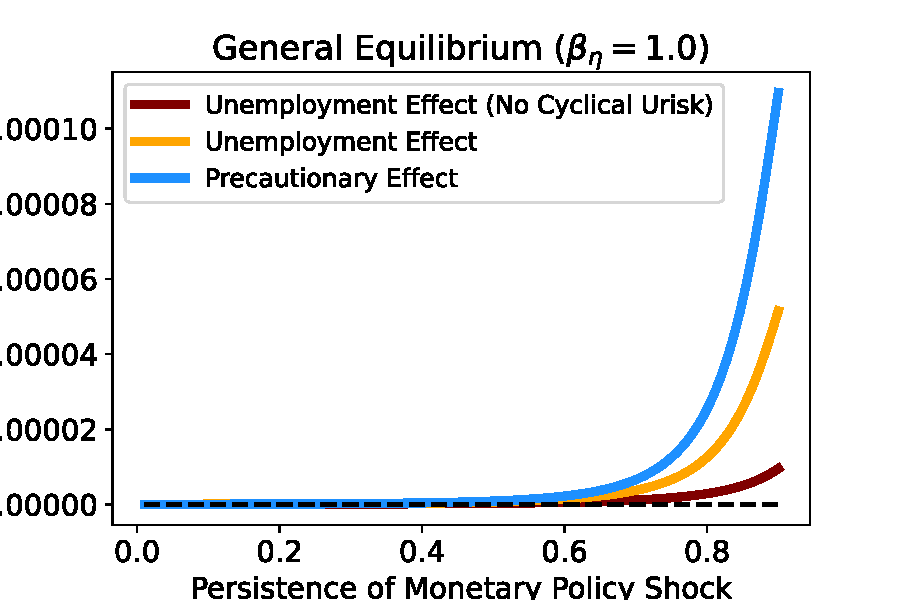
\includegraphics[scale=1.0]{\FigDir/Consumption_Variances_baseline}
    \caption{ Consumption Variance Decomposition }
     \label{fig:Persistence_baseline}
\end{figure}

\begin{figure}{}
    \centering
    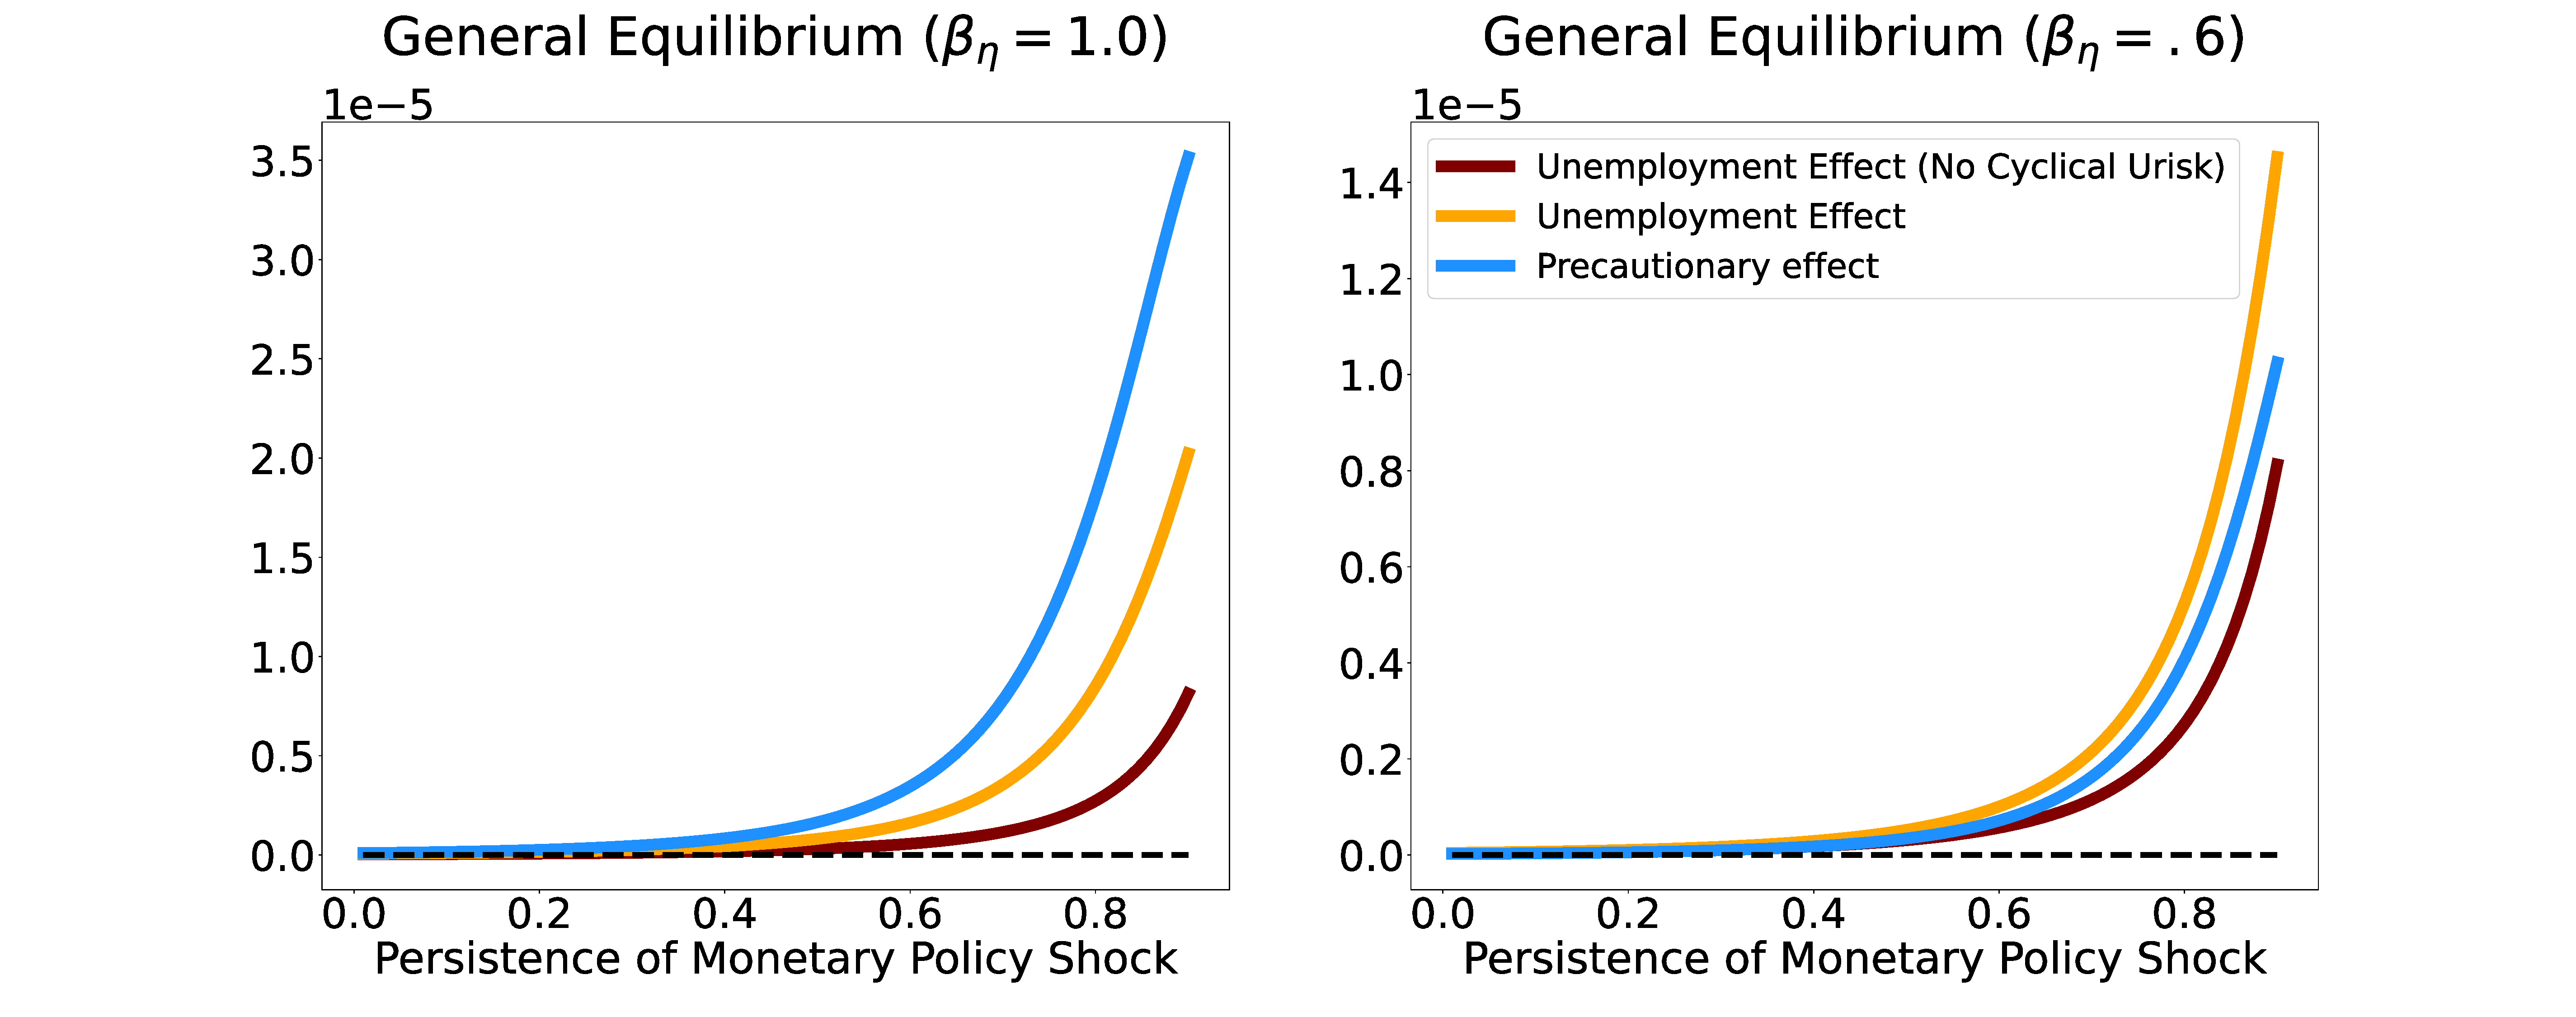
\includegraphics[scale=.16]{\FigDir/Consumption_Variances_G}
    \caption{ Consumption Variance Decomposition (Model with Government Spending)}
     \label{fig:Persistence_Gov}
\end{figure}






\end{document}
